% Template for the submittion to:
%   The Annals of Probability           [aop]
%   The Annals of Applied Probability   [aap]
%   The Annals of Statistics            [aos]
%
%Author: In this template, the places where you need to add information
%        (or delete line) are indicated by {???}.  Mostly the information
%        required is obvious, but some explanations are given in lines starting
%Author:
%All other lines should be ignored.  After editing, there should be
%no instances of ??? after this line.

% use option [preprint] to remove info line at bottom
% journal options: aop,aap,aos
%\documentclass[aos]{imsart}
\documentclass{imsart}

\usepackage{amsthm,amsmath,natbib}
%\RequirePackage[dvips]{hyperref}

% use this package if hyperref and natbib is used:
%\RequirePackage{hypernat}

% provide arXiv number if available:
%\arxiv{math.PR/0000000}

% put your definitions there:
\startlocaldefs
\usepackage{algorithm}
\usepackage{algorithmic,amssymb}
\usepackage{graphicx,xcolor}
\usepackage{subfigure}
%\usepackage[boxed]{algorithm2e}


\renewcommand{\algorithmicrequire}{\textbf{Input:}}
\renewcommand{\algorithmicensure}{\textbf{Output:}}
\renewcommand{\algorithmiccomment}[1]{\# #1}

\newcommand{\argmax}{\mathop{\mathrm{argmax}}}
\newcommand{\argmin}{\mathop{\mathrm{argmin}}}
\newcommand{\minimize}{\mathop{\mathrm{minimize}}}
\newcommand{\maximize}{\mathop{\mathrm{maximize}}}

\newcommand{\todo}{\textcolor{red}{\textbf{To do: }}}

\newcommand{\real}{\mathbb{R}}
\newcommand{\Pp}{{\mathbb P}}
\newcommand{\Ee}{{\mathbb E}}
\newcommand{\lips}{{\cal L}}
\newcommand{\tube}{\mathrm{Tube}}
\newcommand{\sphere}[1]{O^{#1-1}}
\newcommand{\dimens}{\text{dim}}
\newcommand{\cone}{\text{Cone}}
\newtheorem{theorem}{Theorem}
\newtheorem{lemma}[theorem]{Lemma}
\newtheorem{cor}[theorem]{Corollary}
\newcommand{\XK}{K_X}
\newcommand{\norm}[1]{\lVert #1 \rVert}
\newcommand{\innerp}[2]{\langle #1 , #2 \rangle}
%\newcommand{\qed}{\hfill $\Box$\newline}

\newcommand{\grad}{\nabla}
\newcommand{\V}{\mathcal{V}}\endlocaldefs
\newcommand{\K}{\mathcal{K}}
\newcommand\tf{\widetilde{f}}
\newcommand{\pen}{\mathcal{P}}
\newcommand{\vecsp}{\mathcal{L}}
\newcommand{\gstar}{g^*}

\newcommand{\jonathan}[1]{{\color{blue}  #1}}

\begin{document}

\begin{frontmatter}

% "Title of the paper"
\title{A significance test in forward stepwise regression}

%%%
%%% \runtitle{} - I don't know what this is
%%%

% indicate corresponding author with \corref{}
%\author{\fnms{Jonathan} \snm{Taylor}\corref{Jonathan E. Taylor}\ead[label=e1]{jonathan.taylor@stanford.edu}\thanksref{t1}
%\and \fnms{Joshua} \snm{Loftus}}
%\thankstext{t1}{Supported in part by NSF grant DMS 1208857 and AFOSR grant 113039.}

\affiliation{Stanford University}

\address{Department of Statistics\\  Stanford University\\ Sequoia
Hall \\390 Serra Mall\\ Stanford, CA 94305, U.S.A.\\ }
%\printead{e1}}

%%%
%%% \runauthor{Taylor} - I don't know what this is
%%%

\begin{abstract}
% perhaps de-emphasize group lasso and emphasize forward stepwise?
  We extend the methods developed by \cite{significance:lasso} and
  \cite{tests:adaptive} on significance tests for penalized
  regression to stepwise model selection by iteratively applying
  the global null hypothesis test on the residual in a forward stepwise
  procedure. While not fully theoretically justified, the resulting method
  has the computational strengths of stepwise selection and partially
  solves the problem of inflated test statistics due to model selection.
  We illustrate the flexibility of this method by applying it to
  novel specialized applications of forward stepwise to a hierarchically
  constrained interactions model and generalized additive models.
\end{abstract}

%%%
%%% - Gotta change these??????????
%%%
\begin{keyword}[class=AMS]
\kwd[Primary ]{62M40}
%\kwd{}
\kwd[; secondary ]{62H35}
\end{keyword}

\begin{keyword}
\kwd{forward stepwise}
\kwd{model selection}
\kwd{significance test}
\end{keyword}

\end{frontmatter}


\section{Introduction}
\label{sec:intro}

Forward stepwise regression is a classical model selection procedure
that begins with an empty model and sequentially adds the best predictor
variable in each step. The usual $\chi^2$ and $F$-tests for significance
fail when a model has been selected this way and tend to be
anti-conservative unless they are computed on a held-out validation
dataset. In the lasso setting, \cite{significance:lasso} derived
a novel test statistic and its asymptotic null distribution, making
possible valid inferences after model selection using the full data.
\cite{tests:adaptive} modified and extended those results to the
group lasso \citep{grouplasso} and other penalized regression
problems, but only under the global null hypothesis.
One of the strengths of these test statistics is that they can be
used for valid significance testing when computed on the same
data used for model selection, eliminating the need for data splitting or for situations in which
data splitting is not appropriate.
The present work iteratively applies the global null test
of \cite{tests:adaptive} for each step in forward stepwise selection,
and works out some of the details necessary for
models with grouped variables. The resulting method can
be more statistically efficient than validation on held-out data, and
more computationally efficient than penalized methods with
regularization parameters chosen by cross-validation.


In Section~\ref{sec:stepwise} we establish notation and describe the
forward stepwise algorithm used in most of the paper.
Section~\ref{sec:testing}  reviews some recent work on
post-selection inference: \cite{significance:lasso,tests:adaptive,lasso:fixed}
relevant to our work here, and we describes a general framework
for post-selection inference based on quadratic comparisons.
Simulation results in Section~\ref{sec:simulations} show
empirically that our method performs well in settings where forward
stepwise itself performs well, and that
various stopping rules using our test statistic--including
some from \cite{sequential:fdr}--appear promising. In
Section~\ref{sec:applications} we apply
the method to several variants of forward
stepwise tailored to models with interactions and generalized additive
models, as well as to a real data example.
(\todo Change this paragraph if necessary as the sections are completed)
%%%%%%%%%%%%%%%%%%%%%%%%%%%%%%%%%%%%%%%%%%%%%%%%%%%%
%%%%%%%%%%%%%%%%%%%%%%%%%%%%%%%%%%%%%%%%%%%%%%%%%%%%
%%%%%%%%%%%%%%%%%%%%%%%%%%%%%%%%%%%%%%%%%%%%%%%%%%%%

\section{Forward stepwise model selection}
\label{sec:stepwise}

\subsection{Background and notation}

\begin{figure}
\begin{center}
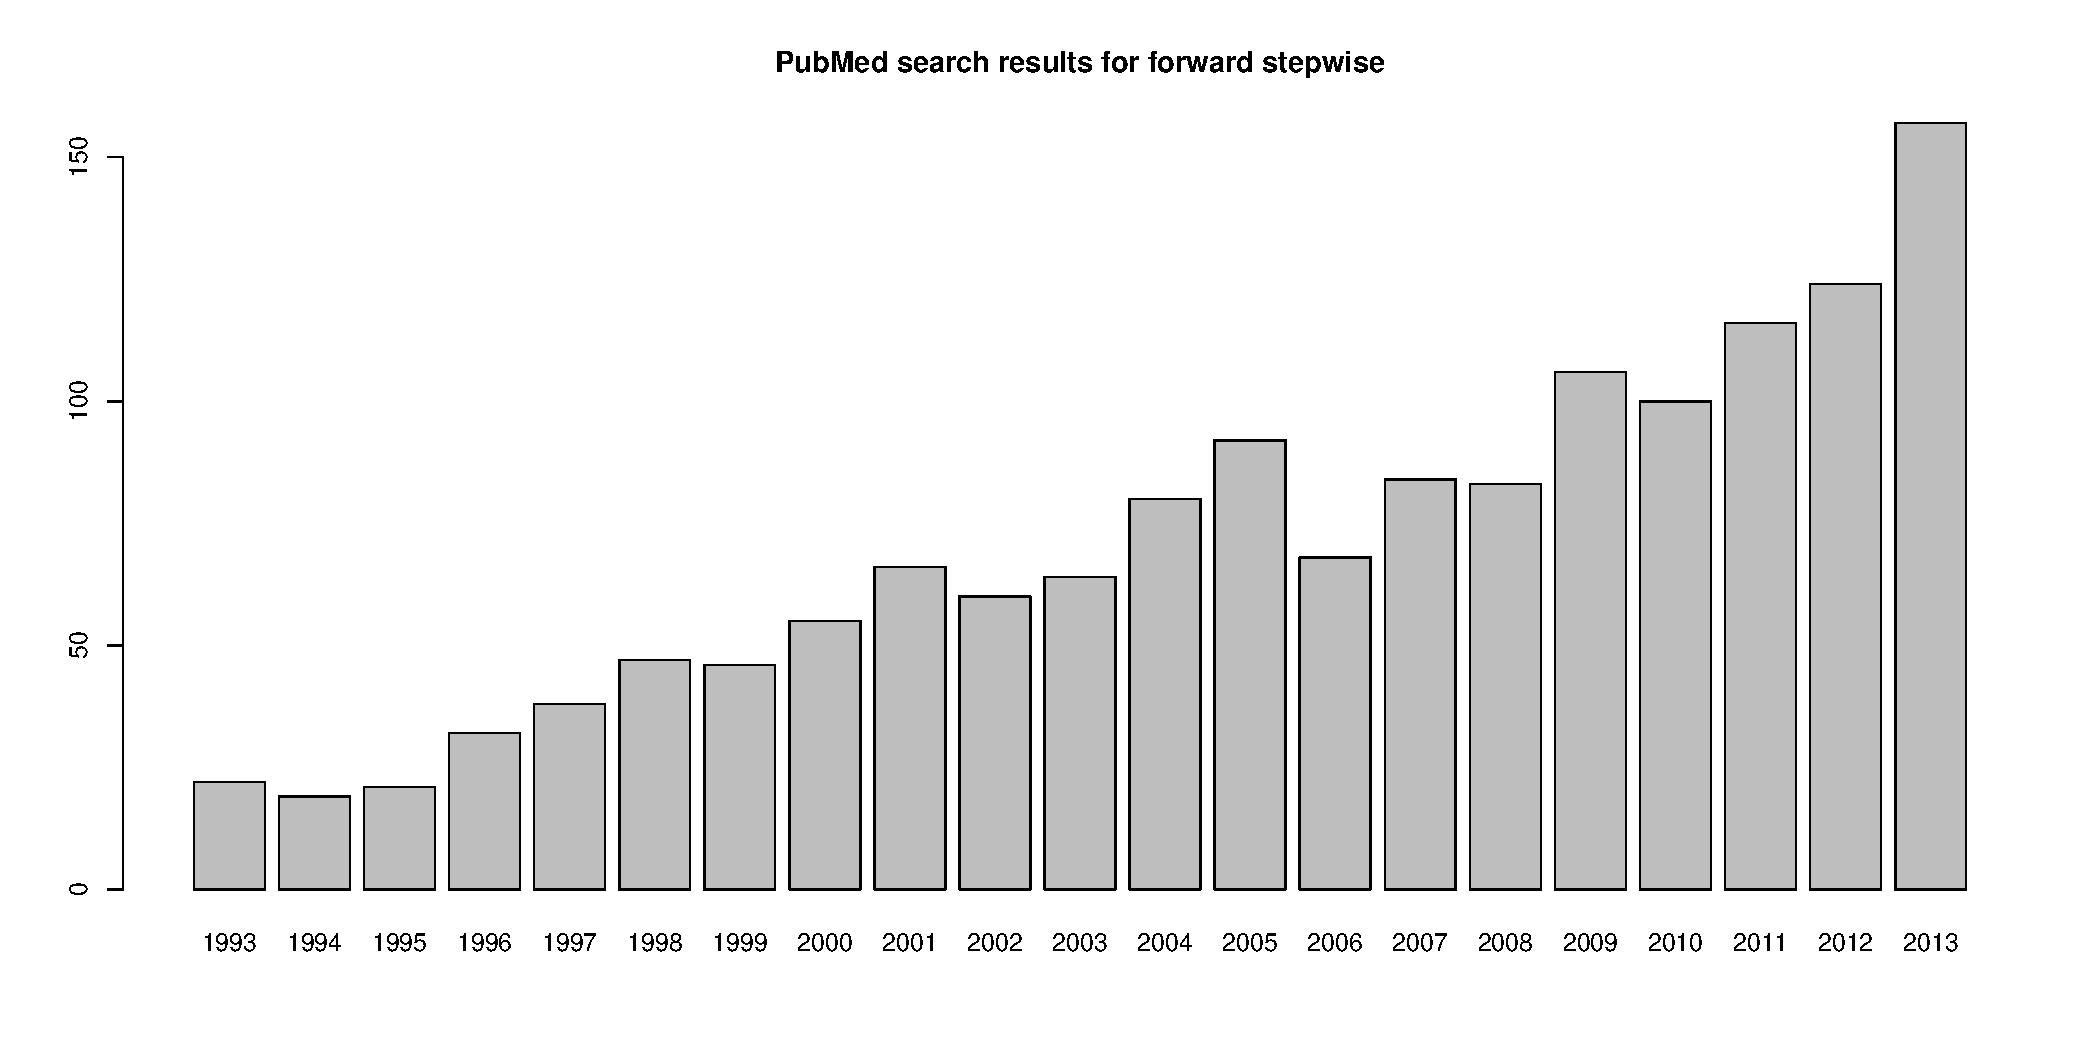
\includegraphics[width=0.9\textwidth]{../figs/pubmed.pdf}
\caption{\small \it Forward stepwise enjoys widespread use among
practitioners}
\label{fig:pubmed}
\end{center}
\end{figure}


As a classical method dating back about half a century
(see \cite{classical:selection} for a review),
forward stepwise regression has not received much attention in
recent years in the theoretical statistics community. But it continues
to be widely used by practitioners.
For example, search results on PubMed for forward stepwise
(summarized in Figure~\ref{fig:pubmed}) show that many recent
papers mention the method and there is an increasing trend over time.
Its popularity among researchers continues despite the fact that it
invalidates inferences using the standard $\chi^2$ or $F$-tests.


Some attempts to address this issue include Monte Carlo
estimation of tables of adjusted $F$-statistic values \citep{mc:ftoenter},
and permutation statistics \citep{permutation:stop}. Aside from the works
this paper is based on, there have been other recent attempts to do
inference after model selection. Most of these make use of subsampling
\citep{meinshausen:buhlmann} or data splitting \citep{wasserman:roeder}.
Our approach allows use of the full data and does not require the
extra computation involved in subsampling.
Before describing the full approach we first introduce notation and
specify our implementation of forward stepwise, which is slightly
different from the most commonly used versions.


We allow forward stepwise selection to add groups of variables in each
step, not only in the case of binary encoding for categorical
variables but also for any grouping purpose. For example, groups of
variables may be pre-designated factors such as expression
measurements for all genes in a single functional pathway.
To emphasize this we use $g, h$ as indices rather than the usual
$i, j$ throughout. Since single variables can be considered groups of
size 1, our general exposition includes non-grouped situations as a special
case. Our variant of forward stepwise uses a different method than
usual for choosing which group to add because we are using the
same objective in the forward stepwise procedure that was used to
derive the test statistics in penalized regression settings.

Denote $y \in \real^n$ for $n$ i.i.d. measurements of the outcome variable.
Let an integer $G \geq 2$ be the number of groups of explanatory variables.
For each $1 \leq g \leq G$ the design matrix encoding the
$g$th group is the $n \times p_g$ matrix denoted $X_g$, where $p_g$ is
the number of individual variables or columns in group $g$.
% Do we need to assume $p_g \ll n$ or $\text{rank}(X_g) = p_g$?
When a group encodes a categorical variable as binary indicators for the
levels of that variable, by default we use the full encoding with a column for every
level. Although this introduces collinearity, our method does not require
the design matrix to have full rank.


Define $p = \sum_{g=1}^Gp_g$,
the total number of individual variables, so $p = G$ in the
case where all groups have size 1. Let $X$ be the matrix constructed
by column-binding the $X_g$, that is  
%%%%%%%%%%%%%%%%%%%%%%%%%%%%%%%%%%%%%%%%%%%%%%%%
\begin{equation*}
X = \begin{pmatrix} X_1 & X_2 & \cdots & X_G  \end{pmatrix}
\end{equation*}
%%%%%%%%%%%%%%%%%%%%%%%%%%%%%%%%%%%%%%%%%%%%%%%%
For convenience, we assume throughout that the individual columns of $X$ are scaled to
have unit 2-norm (we do not scale groups, this is accomplished later
by weighting).
With each group we associate the $p_g \times 1$ coefficient vector
$\beta_g$, and write $\beta$ for the $p \times 1$ vector constructed
by stacking all of the $\beta_g$ in order.  Finally, our model for the
response is
%%%%%%%%%%%%%%%%%%%%%%%%%%%%%%%%%%%%%%%%%%%%%%%%
\begin{equation}
\begin{aligned}
\label{eq:gmodel}
y | X& = X \beta + \sigma \epsilon \\
   & = \sum_{g=1}^G X_g \beta_g + \sigma \epsilon
\end{aligned}
\end{equation}
%%%%%%%%%%%%%%%%%%%%%%%%%%%%%%%%%%%%%%%%%%%%%%%%
where $\epsilon$ is noise. We assume Gaussian noise
$\epsilon | X \sim N(0, \Sigma)$ with known covariance matrix $\Sigma$.


The model \eqref{eq:gmodel} is underdetermined when $p > n$.
In such cases it still may be possible to
estimate $\beta$ well if it is sparse--that is, if it has few nonzero
entries. In the rest of this paper we refer to variable groups $X_g$
as noise groups if $\beta_g$ is a zero vector and as true or signal
groups if $\beta_g$ has any nonzero entries. We refer to the number
of such nonzero groups as the \textit{sparsity} of the model, and
denote this $k := \# \{ g : \beta_g \neq 0 \}$.

Before we describe the forward stepwise procedure we require one last
ingredient. To each group of variables we assign a weight $w_g$. These
weights act like penalties or costs, so increasing $w_g$ makes it
more difficult for the group $X_g$ to enter the model. The
modeler can choose weights arbitrarily, but we mostly use one
particular choice, based on $p_g$, that we discuss later. With this we
are ready to describe the forward stepwise procedure.


\subsection{Description of the algorithm}

First, the user must specify the maximum number of steps allowed,
which we denote \textit{steps} (consistent with the \textit{R} function
for stepwise). To enable our test statistic computations,
\textit{steps} should be at most $\min (n, G) - 1$, but it is
computationally desirable to set it as low as possible while still being
larger than the (unknown) sparsity of $\beta$.
This way forward stepwise has a chance of recovering all the nonzero
coefficients of $\beta$ and then terminating without performing much
additional computation.
In our implementation we treat the active set $A$ as an ordered list to easily track the order of groups entering the model.

% \begin{algorithm}
% \DontPrintSemicolon
% \KwData{An $n$ vector $y$ and $n \times p$ matrix $X$ of $G$ groups of variables}
% \KwResult{Active set $A$ of variable groups included in the model}
% \SetKwFunction{lsfitResidual}{lsfitResidual}
% \caption{\small \it Forward stepwise procedure with groups and weights}
% \BlankLine
% $A \gets \emptyset$\;
% $A^c \gets \{ 1, \ldots, G \}$\;
% $r_0 \gets y$\;
% \For{$s \gets 1$ \KwTo $steps$}{
%   $g^* \gets \argmax_{g \in A^c} \{ \norm{X_g^T r_{s-1}}_2 / w_g \}$\;
%   $P \gets I - X_{g^*}X_{g^*}^\dagger$\;
%   $A \gets A \cup \{ g^* \}$\;
%   $A^c \gets A^c \backslash \{ g^* \}$\;
%   \For{$g \in A^c$}{
%     $X_g \gets P X_g$\;
%   }
%   $r_s \gets P r_{s-1}$\;
% }
% \KwRet{$A$}
% \label{algo:fs}
% \end{algorithm}

\jonathan{Is $r_0=0$ or $y$? Should be defined in the algorithm. I also put a $y$ in below which I'm not sure
is correct or not. }

\begin{algorithm}
  \caption{Forward stepwise variant with groups and weights}
  \label{algo:fs}
  \begin{algorithmic}[1]
    \REQUIRE An $n$ vector $y$ and $n \times p$ matrix $X$ of $G$ variable groups with weights $w_g$
    \ENSURE Ordered active set $A$ of variable groups included in the model at each step
    \STATE $A \gets \emptyset$, $A^c \gets \{ 1, \ldots, G\}$
    \FOR{$s=1$ to $steps$}
    \STATE $g^* \gets \argmax_{g \in A^c} \{ \norm{X_g^T(y- r_{s-1})}_2 / w_g \}$
    \STATE $P_{g^*} \gets I_{n\times n} - X_{g^*}X_{g^*}^\dagger$
    \STATE $A \gets A \cup \{ g^* \}$, $A^c \gets A^c \backslash \{ g^* \}$
    \FORALL{$h \in A^c$}
      \STATE $X_h \gets P_{g^*} X_h$
    \ENDFOR
    \STATE $r_s \gets P_{g^*} r_{s-1}$
    \ENDFOR
    \RETURN $A$
  \end{algorithmic}
\end{algorithm}

The active set $A$ contains variable groups chosen to be included in
the model. Fitting $\hat \beta$ can be done by tracking the individual
fits and projections, or by simply fitting a linear model on the submatrix
of $X$ corresponding to $A$. 
We now use forward stepwise to refer specifically to
Algorithm~\ref{algo:fs} unless otherwise specified. Note that other
implementations of forward stepwise use different criteria for choosing
the next variable to add, such as the correlation with the residual.
Since we do not renormalize the columns after projecting the covariates
(lines 6 to 8 above), and since we have weights, we are generally not computing
correlations unless the design matrix is orthogonal and all weights are 1. We could
renormalize the columns, though we choose not to.
There are advantages and disadvantages to both criteria which we do not
discuss. Our choice was motivated by the group lasso result in
\cite{tests:adaptive}, but we believe other criteria can be handled
with appropriate modifications.

\subsection{Performance of forward stepwise}

Among model selection procedures, forward stepwise is one which performs
variable selection: from a potentially large set of variables it chooses
a subset to include in the model. The most general form of variable
selection is  "best-subset" selection, a procedure which searches among
all $2^G$ subsets of $G$ variable groups and picks the best model.
This exhaustive search is computationally infeasible when $G$ is
large, and when possible it still
runs the risk of over-fitting unless model complexity is
appropriately penalized (as in \eqref{eq:subsetregress} below).
Forward stepwise produces a much
smaller set of potential models, with cardinality at most
\textit{steps}. However
it is a greedy algorithm, so the set of models it produces may not
contain the best possible model. This is an inherent shortcoming of
forward stepwise procedures and should be kept in mind when choosing
between model selection methods.

So far we have left open the question of choosing among the models in
the forward stepwise sequence, i.e. when to stop stepping
forward. Some approaches for this problem can be posed as optimization
criteria which stop at the step minimizing
\begin{equation}
\begin{aligned}
\label{eq:subsetregress}
\frac{1}{2} \| y - X \beta_s \|_2^2 + \lambda \pen(\beta_s)
\end{aligned}
\end{equation}
(\todo describe construction of $\beta$ after finding $A$)
where we have written $\{ \beta_s : s = 1, \ldots, steps \}$ as
the sequence of models outputted by forward stepwise. The function
$\pen(\beta)$ is a penalty on model complexity usually taken to be the
number of nonzero entries of $\beta$. Proposals for $\lambda$ include
2 ($C_p$ of \cite{CP}, AIC of \cite{AIC}), $\log(n)$ (BIC of \cite{BIC}), and
$2\log(p)$ (RIC of \cite{RIC}). Stopping rules based on classical test
statistics have also been used, so it is natural to consider using
the new test statistics of \cite{significance:lasso} or
\cite{tests:adaptive}
to choose a model. \cite{sequential:fdr} examined some stopping rules
using the asymptotic p-values of \cite{significance:lasso} and showed
their stopping rules control false discovery rate--the expected
proportion of noise variables among variables declared significant
\citep{fdr}. We explore this further in Section~\ref{sec:simulations}.

Although forward stepwise is a greedy algorithm producing a
potentially sub-optimal sequence of models, under favorable conditions
it can still perform well. There is a small segment of the
compressed sensing literature \citep{donoho:pursuit, cai:wang:omp}
with results stating that forward stepwise (often referred to in that
literature as Orthogonal Matching Pursuit or OMP) can exactly select
the true model
under some stringent conditions involving quantities like the sparsity
of the true model and the coherence of the design matrix. The
coherence $\mu(X)$ of a matrix $X$ with columns scaled to have unit
2-norm is defined as

\begin{equation}
  \mu := \mu(X) = \max_{i \neq j} \{ | \innerp{ X_i }{ X_j } | \}
\end{equation}

Recalling that $k$ is the sparsity of $\beta$, typical results in this
literature say that if $k < (1/\mu + 1)/2$ and the nonzero
coefficients of $\beta$ are sufficiently large then forward stepwise
recovers $\beta$ with high probability. The coherence condition is
necessary to guarantee exact recovery \citep{cai:wang:xu:sharp} in the
sense that it is possible to construct counterexamples with
$k = (1/\mu + 1)/2$. We refer the reader to the literature for details.
For our purposes the
conditions required to guarantee exact recovery are usually too
stringent. Simulations show empirically that forward
stepwise can work well even when it is not working perfectly, and that
it does so under a wide range of conditions.


\begin{figure}
\begin{center}
\subfigure[Ternary design]{
\label{fig:fsternary}
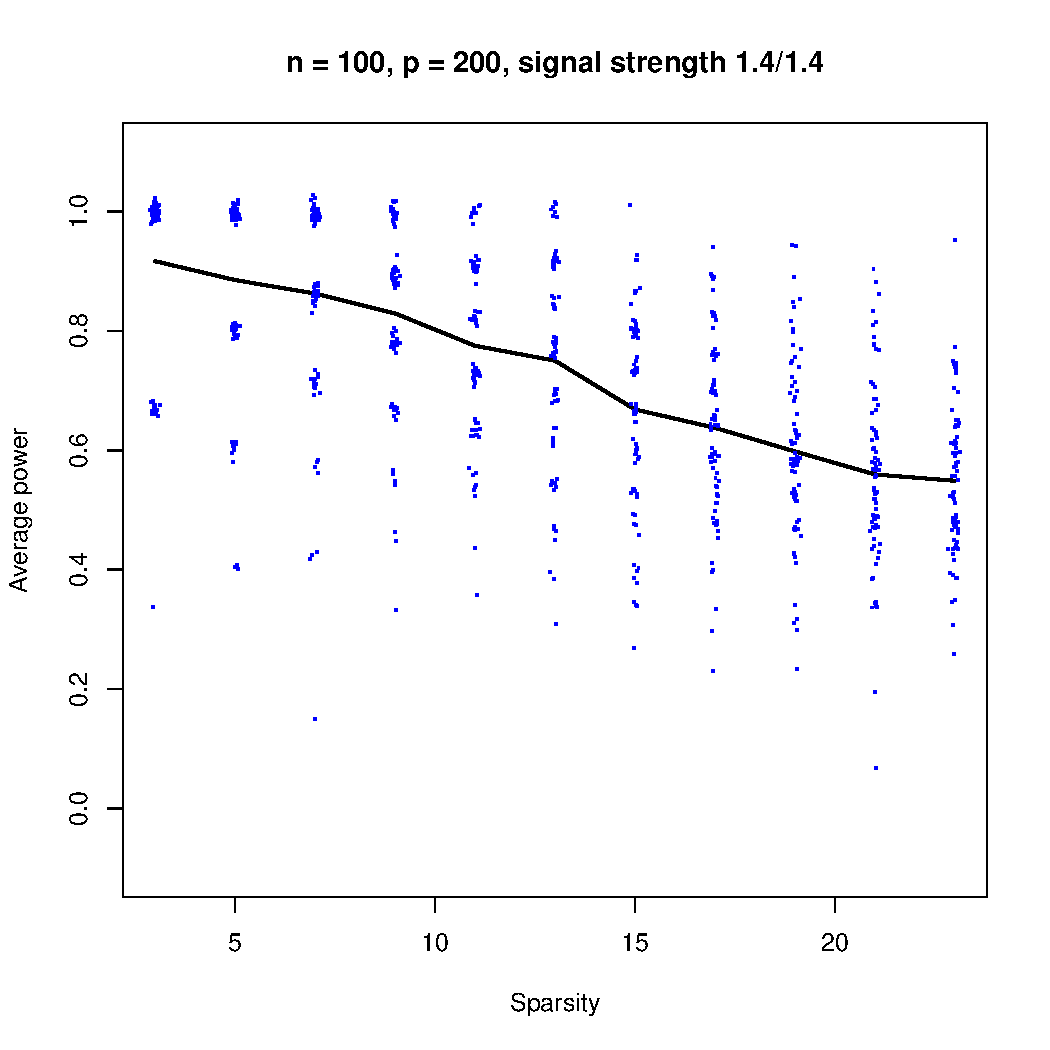
\includegraphics[width=0.5\textwidth]{../figs/fwdstep/ternary_p2n_n100_lower1p4_upper1p4.pdf}}
\hspace{-15pt}
\subfigure[Gaussian design with correlation]{
\label{fig:fsgausscorr}
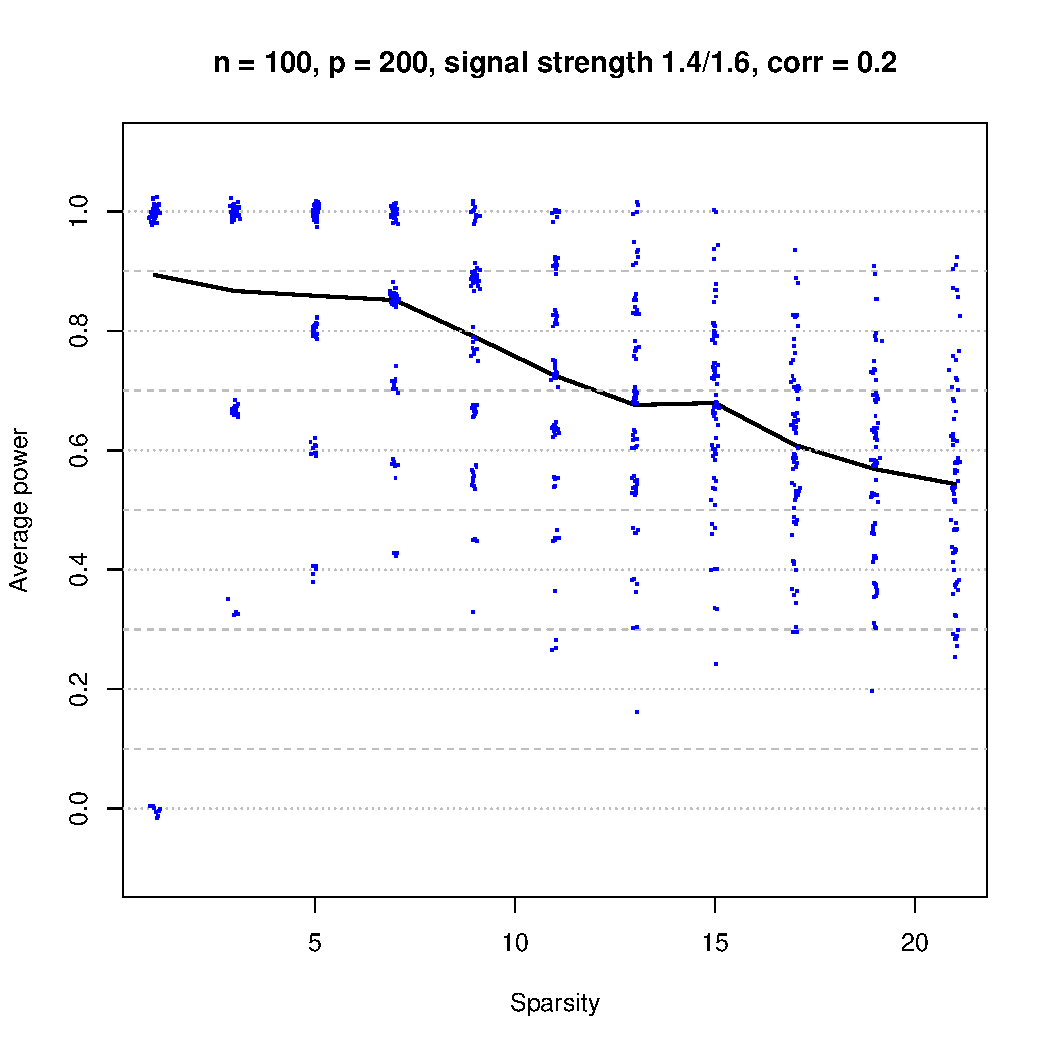
\includegraphics[width=0.5\textwidth]{../figs/fwdstep/gaussian_p2n_n100_lower1p4_upper1p6_corr0p2.pdf}}
\caption{\small \it The left panel shows the results of the simulation
  using design matrices with i.i.d. ternary entries taking values $0,
  \pm 1$ with equal probability. The left panel shows the results
  with design matrices of standard Gaussian entries with
  equi-correlation of 0.2. }
\label{fig:fwdstepsim}
\end{center}
\end{figure}

\jonathan{Is average power the same as TPR (or, more correctly, TPP)?}


For various sparsity levels $k$, Algorithm~\ref{algo:fs} was run on
various data sets with \textit{steps} equal to $k$ and the ``average
power'' was calculated as the number of true variables in the active
set after $k$ steps divided by $k$:
$$
\text{Power}_k = \frac{\# \left\{g: g \in A_k, \beta_g \neq 0\right\}}{k}.
$$ (\todo Make this consistent with
$\gamma$ in simulations section)
Nonzero coefficients had magnitude
in a range of multiples of $\gamma := \sqrt{2\log(G)}$, e.g. in $[1.4
\gamma, 1.6 \gamma]$. Results are shown in
Figure~\ref{fig:fwdstepsim}. After computing the
coherence of these design matrices, some calculations show the required
sparsity level to guarantee exact recovery in these situations is
about 2 or smaller, and the required nonzero coefficient magnitude is
likely in the range of 10 to 100 times $\gamma$. These simulations are far
from the stringent conditions required by theory to guarantee perfect
recovery, but the performance, while not perfect, may still be good
enough for some purposes.



%%%%%%%%%%%%%%%%%%%%%%%%%
%%%%%%%%%%%%%%%%%%%%%%%%%

\section{Significance testing: from lasso to group lasso}
\label{sec:testing}

\todo Reorganize and update this section \\

In the ordinary least squares setting, a significance test for a
single variable can be conducted by comparing the drop in residual
sums of squares (RSS) to a $\chi^2_1$ distribution. Similarly, when
adding a group of $k$ variables we can compare the drop in RSS to a
$\chi^2_k$ random variable. This generally does not work when the
group to be added has been chosen by a method that uses the data \cite{olshen:flevel},
and in particular it fails for forward stepwise procedures adding
the ``best'' (e.g. most highly correlated) predictor in each step. In
that case, the test statistic (drop in RSS) does not match the
theoretical null distribution even when the null hypothesis is
true. \cite{significance:lasso} introduced a new test statistic based
on the knots in the lasso solution path. They derived a simple
asymptotic null distribution, proved a type of convergence under broad
``minimum growth'' conditions, and demonstrated in simulations that
the test statistic closely matches its asymptotic distribution even in
finite samples.  That work marked an important advance in the problem
of combining inference with model selection.  \cite{tests:adaptive}
extended that work to the group lasso \citep{grouplasso} and other
problems, and modified the test statistic to one with an exact finite
sample distribution under the global null hypothesis.


Writing $\hat \beta(\lambda)$ for the lasso solution for a fixed value of $\lambda$, we recall
the following facts summarized in \cite{significance:lasso,tibshirani_lasso_uniqueness}.

\begin{itemize}

  \item The vector valued function $\hat \beta(\lambda)$ is a
    continuous function of $\lambda$. For the lasso path, the
    coordinates of $\hat \beta(\lambda)$ are piecewise linear with
    changes in slope occurring at a finite number of $\lambda$ values
    referred to as \emph{knots}. 
    \item The knots depend on the data and are
    usually written in order $\lambda_1 \geq \lambda_2 \geq \cdots
    \geq \lambda_r \geq 0$. 

\end{itemize}

The covariance test (assuming $X$'s columns are of length one and $\Sigma = \sigma^2 I$ is at the
first step by
\begin{equation}
\label{eq:covtest}
T_1 = \frac{\lambda_1(\lambda_1-\lambda_2)}{\sigma^2} \overset{n,p \to \infty}{\to} \text{Exp}(1).
\end{equation}
In \cite{tests:adaptive} it is pointed out 
\begin{equation}
\label{test:exact}
\exp\left(- \frac{\lambda_1(\lambda_1-\lambda_2)}{\sigma^2} \right) \approx \frac{1 - \Phi(\lambda_1/\sigma)}{1 - \Phi(\lambda_2 / \sigma)} \overset{D}{=} \text{Unif}(0,1).
\end{equation}
Further, the above test statistic can be understood as the survival function of $\lambda_1 = \|X^Ty\|_{\infty}$
{\em conditional} on which variable achieves $\lambda_1$ as well as its sign.
The limiting results about later steps in \cite{significance:lasso} can (formally) be interpreted as
recursively applying $T_1$ to the variables that had not previously been selected by LARS.

In the setting of grouped variables, we use an analogous test statistic to
the right hand side of \eqref{test:exact}. The test statistic is presented as an example
in \cite{tests:adaptive} though we re-derive it here in simpler form. The test draws inspiration
from the group LASSO.

The \emph{group lasso estimator} is a solution to the following convex
problem
%%%%%%%%%%%%%%%%%%%%%%%%%%%%%%%%%%%%%%%%%%%%%%%%
\begin{equation}
\begin{aligned}
\label{eq:gsoln}
\displaystyle \hat \beta_\lambda = \argmin_{\beta \in \real^p} \frac{1}{2} \| y - X \beta \|_2^2 +
   \lambda \sum_{g=1}^G w_g \| \beta_g \|_2
\end{aligned}
\end{equation}
%%%%%%%%%%%%%%%%%%%%%%%%%%%%%%%%%%%%%%%%%%%%%%%%
The parameter $\lambda \geq 0$ enforces sparsity in groups: for large
$\lambda$ most of the $\beta_g$ will be zero vectors. The weights
$w_g$ are usually taken to be $\sqrt {p_g}$ to normalize the penalty
across groups.  Note that this includes the usual lasso estimator as a
special case when all of the groups are of size 1, since then the
penalty term is the $L^1$-norm of $\beta$. 

There is a largest value of $\lambda$ such that $\hat{\beta}_{\lambda}=0$ which corresponds to $\lambda_1$
in the LASSO setting:
\begin{equation}
\label{eq:lammax}
\lambda_1^{\text{group}} = \max_{g} \frac{1}{w_g}\|X_g^Ty\|_2 . 
\end{equation}
Formally, the value above is just the dual norm of the penalty
$$
{\cal P}(\beta) = \sum_{g=1}^G w_g \| \beta_g \|_2
$$
hence it can be expressed as
\begin{equation}
\label{eq:lammax}
\lambda_1^{\text{group}} = \max_{g} \frac{1}{w_g}\|X_g^Ty\|_2 = \frac{1}{w_{g^*}}\eta_{g^*}^TX_{g^*}^Ty . 
\end{equation}
where $g^*$ is the group that achieves the max and 
$\eta_{g^*} = X_{g^*}^Ty / \|X_{g^*}^Ty\|_2$ is the $\ell_2$ unit vector that achieves $\|X_{g^*}^Ty\|_2$.

%%%%%%%%%%%%%%%%%%%%%%%%%%%%%%%%%%%%%%%%%%%%%%%%
%%%%%%%%%%%%%%%% Related works %%%%%%%%%%%%%%%%%
%%%%%%%%%%%%%%%%%%%%%%%%%%%%%%%%%%%%%%%%%%%%%%%%


\begin{figure}
\label{fig:polytope}
\begin{center}
\resizebox{!}{3in}{\input{../figs/polytope.pdf_tex}}
\end{center}
A polytope selection event. Solving the LASSO \eqref{eq:lasso} for a fixed value
of $\lambda$ yields both an active set $\hat{E}(y)$ and a collection of signs of 
active variables $z_{\hat{E}(y)}$. The event $\{y: (\hat{E}(y), z_{\hat{E}(y)}) = (E, z_E)\}$
can be written as a set of affine constraints.
\end{figure}

\subsection{Selection events}

The approach to post-selection inference described \cite{lasso:fixed}
describes the selection event for the LASSO as a convex polytope stylized
in Figure \ref{fig:polytope}. If all of our groups were of size 1, then
the event that we observe a given set of variables
in the forward stepwise path (with their signs as they enter) would also
be described by a set of affine inequalities. This is described in more detail in \cite{exact:lars}.

After selection, exact inference for a (randomly) chosen contrast $\eta(y)^T\mu$ of the mean vector
$\mu$ is carried by considering the conditional distribution of 
\begin{equation}
y \sim N(\mu, \sigma^2 I) \bigl| Ay \leq b.
\end{equation}
See \cite{lasso:fixed,exact:lars} for further details.

In the grouped variables setting, however, the event that $g^*(y)$, the first
group chosen, is equal to some fixed group $g$ is generally not described by
a set of affine constraints. The event can be described as
\begin{equation}
\label{eq:first:quadratic}
\begin{aligned}
\{g^*(y)=g\} &= \{ \|X_g^Ty\|_2 /w_g \geq \|X_h^Ty\|_2 /w_h , \ \forall h \neq g\} \\
&=  \{ y^T(X_g^TX_g)y / w_g - y^T(X_h^TX_h)y / w_h, \ \forall h \neq g\} \\
\end{aligned}
\end{equation}

Hence, our selection event can be expressed as 
the intersection of a list of quadratic inequalities. This non-affine selection event is stylized in Figure
\ref{fig:curved}.
In this section, we consider an arbitrary selection procedure
$S$ that returns one of a set of possible outcomes $s \in {\cal S}$ by a set of quadratic inequalities.
That is, for all possible outcomes $s \in {\cal S}$:
\begin{equation}
\label{eq:selection}
\begin{aligned}
\{S(y)=s\} = \cap_{i \neq I(s)} \{y: y^TQ_iy + a_i^Ty\leq b_i \}.
\end{aligned}
\end{equation}

The quadratic forms are not assumed non-negative definite, but we can, without loss of generality
assume they are symmetric.
As in \cite{lasso:exact} we will be interested in some randomly chosen contrast
$\eta(S(y))^T\mu$. In our grouped selection procedure, the procedure $S(y)=g^*(y)$
and $\eta$ is typically 
$$
\eta(S(y)) = \eta(g^*(y)) = \frac{X_{g^*(y)}^Ty}{\|X_{g^*(y)}^Ty\|_2}.
$$

Having fixed $\eta$, we must slice through the selection event along a ray with direction $\eta$ that passes through $y$. 
That is, we need to find
$$
\begin{aligned}
\left\{t: S(y+t \cdot \eta)=s \right\} &= \cap_{i \in I(s)} \left\{t: (y+t \cdot \eta)^T Q_i (y+t \cdot \eta) + a_i^T(y+t \cdot \eta) \leq b_i\right\}. \\
\end{aligned}
$$

\begin{figure}
\label{fig:curved}
\begin{center}
\resizebox{!}{3in}{\input{../figs/curved.pdf_edit_tex}}
\end{center}
A generic selection event, given by the intersection of a list
of quadratic inequalities. Note that the event need not be simply connected. \end{figure}

The slice for any particular inequality is
$$
\begin{aligned}
\lefteqn{
\left\{t: (y+t\eta)^T Q_i (y+t \cdot \eta) + a_i^T(y+t \cdot \eta) \leq b_i\right\}} \\
 & \qquad = \left\{t: t^2 \cdot \eta^TQ_i\eta + t \cdot(2 y^TQ_i\eta + a_i^T\eta) + y^TQ_iy + a_i^Ty - b_i \leq 0 \right\} \\
\end{aligned}
$$
This can be computed easily, and results in either the empty, a single interval (possibly infinite) or the union of 
two disjoint infinite intervals. The intersection over all $I(s)$ is therefore easily computable.
This yields an easily computable form for the slice
\begin{equation}
\label{eq:slice}
\{g^*(y)=g, \eta(g^*(y))=\eta\}.
\end{equation}
In the picture \eqref{eq:curved}, for every $\eta$, the slice \eqref{eq:slice} is a function
of $P_{\eta}^{\perp}y$. This amounts to a proof of the following lemma.

\begin{lemma}
Suppose $S$ is a selection procedure, i.e. a map $S:\real^n \mapsto {\cal S}$
such that for each $s \in S$ \eqref{eq:selection} holds 
and we are given a matrix valued function $X_s \in \real^{n \times p(s)}$ of rank
$k(s)$.
Then, for every $\eta_s \in \real^{p(s)}$ with $\|\eta_s\|_2=1$, the
slice
\begin{equation}
\label{eq:slice:general}
\left\{t: S(y+t \cdot \eta_s)=s, \frac{X_s^Ty}{\|X_s^Ty\|_2}=\eta_s \right\}
\end{equation}
can be described by
a finite union of closed intervals whose endpoints are functions of 
$(P_s^{\perp}y, (P_s- (X_s\eta_s)(X_s\eta_s)^T)y)$ where
$P_s^{\perp}$ is projection on the orthogonal column space of $X_s$.
Denote this set by $E(s, \eta_s, P_s^{\perp}y, (P_s - X_s \eta_s(X_s\eta_s)^T)y)$ and also define
$$
\begin{aligned}
E_+(s, \eta_s, P_s^{\perp}y, (P_s - X_s \eta_s(X_s\eta_s)^T)y) &= \left\{y + t \cdot \eta_s: S(y+t \cdot \eta)=s, \frac{X_s^Ty}{\|X_s^Ty\|_2}=\eta_s \right\} \\
\end{aligned}
$$
\end{lemma}

In turn, this allows to derive a test statistic to test the hypothesis
$H_{0,s}:X_s^T\mu=0$ conditional on $s$ being selected.
\begin{lemma}
\label{eq:test:dbn}
Conditional on $H_{0,s} \cap E_+(s, \eta_s, P_s^{\perp}y, (P_s - \eta_s\eta_s^T)y)$
the following equality holds in distribution
\begin{equation}
\label{eq:chi:truncated}
(X_s\eta_s)^Ty \overset{D}{=} \theta_s \chi_{k(s)} | (X_s\eta_s)^TE_+(s, \eta_s, P_s^{\perp}y, (P_s - \eta_s\eta_s^T)y) 
\end{equation}
where the scale 
$$
\theta_s = \sigma \frac{y^TP_sy}{y^TX_sX_s^Ty}.
$$
\end{lemma}

{\bf Proof:}
For any $s$, decompose the distribution of $y$ as
$$
(Z^{\perp}_s,Z_s) = (P_s^{\perp}y, X_s^Ty).
$$
Under $H_{0,s}:X_s^T\mu=0$, the density of $Z_s$ can be written as
$$
(2 \pi \Sigma_s \sigma^2)^{-k(s)/2} \exp \left(-\frac{1}{2 \sigma^2} z^T\Sigma_s^{-1}z \right)
$$
with $\Sigma_s = X_s^TX_s$.
Transforming to polar coordinates $(R,U)$ yields a density
$$
(2 \pi \Sigma_s \sigma^2)^{-k(s)/2} r^{k(s)-1} \exp \left(-\frac{r^2}{2 \sigma^2} u^T\Sigma_s^{-1}u \right), \qquad r \geq 0, \|u\|_2=1.
$$
Conditioning on $U$ shows that $R=\|X_s^Ty\|_2|U$ has distribution proportional to a $\chi_{r(s)}$. The only thing to determine
is the scale of the $\chi$, which must be $\sigma \|X_s\eta_s\|_2$.

%\subsection{Relation to covariance test}
%
%Consider the simple case for the first covariate to enter the model.
%In this case the covariance test statistic is $T = \lambda_1(\lambda_1 - M)$.
%\todo Does $M = \lambda_2$? Check proof, now that statistic has changed
%
%This is Lemma 5 from \cite{significance:lasso}.
%
%\begin{itemize}
%
%  \item As in LTTT, $T = \lambda_1 (\lambda_1 - M)$ and $M = \lambda_2$
%  \item Convergence to the limiting Exp(1) distribution is too slow
%    \[
%      \frac{P(\chi_k / w_g \geq m + t/m)}{P(\chi_k / w_g \geq m)} \to e^{-t} \text{ as } m \to \infty
%    \]
%    (when the group achieving $\lambda_1$ is group $g$ and has rank $k$)
%  \item The limiting distribution only depends on $T$, but we also observe $M$
%  \item Let's just try the ratio (conditional $\chi_k$ tail probability) evaluated at $T$ and $M$ (it works better)
%  \item Going one step further, instead of using the approximation (see LTTT Proof of Lemma 5)
%    \[
%      \frac{M + \sqrt{M^2+4t}}{2} \approx M + \frac{t}{M}
%    \]
%    we can just use the left hand side
%  \item For $T = \lambda_1(\lambda_1 - M)$ the left hand side simplifies to $\lambda_1$
%  \item Now our p-value is
%    \[
%      \frac{P(\chi_k / w_g \geq \lambda_1)}{P(\chi_k / w_g \geq \lambda_2)}
%    \]   
%\end{itemize}
%
%
%\subsection{Exact p-value calculation}
%
%\todo Complete this section
%
%We now describe how to calculate our p-value, following the discussion of
%group lasso in \cite{tests:adaptive}. For the rest of this section let
%$g = \gstar$ be the index of
%the group attaining the maximum on line 3 of Algorithm~\ref{algo:fs}.
%%\lambda = \norm{X_g^Ty}_2/w_g$ be the value of the maximum, and
%%$r = \text{rank}(X_g)$ be the rank of the maximizing group.
%For a vector $u \in \real^p$, let $u_h$ denote the coordinates
%of $u$ corresponding to the columns of group $h$ in the design matrix $X$.
%We can rearrange the columns of $X$ to group these adjacently, so that
%\[
%u^TX^T = \begin{pmatrix} u_1^T X_1^T & u_2^T X_2^T & \cdots & u_G^TX_G^T \end{pmatrix}
%\]
%One step of the calculation will be to find an orthonormal basis for the
%linear space $\vecsp_g = \{ u \in \real^p : u_g^T X_g^T y = 0, u_h = 0
%\text{ for all } h \neq g \}$ so that we can project orthogonally to
%this space. If $X_g$ is a single column and $X_g^Ty \neq 0$ (which
%should be the case since $g$ maximizes the absolute value of this
%quantity), then the
%space is trivial and the desired orthogonal projection is the identity.
%Otherwise, if $X_g$ has $p_g > 1$ columns the space $\vecsp_g$
%generally has dimension $p_g-1$.
%% have dimension $r-1$ for $r = \text{rank}(X_g)$. This holds except in
%% degenerate cases such as $X_g = 0$ or $r \ll p_g$, but these cases are not
%% likely to occur since $\norm{X_g^T y}_2/w_g$ is supposed to be maximized.
%% We proceed by forming the $n \times p_g$ matrix
%% $X_g - X_g X_g^T y y^T X_g/\norm{X_g^Ty}_2^2$ and performing Gram-Schmidt
%% on the first $r-1$ columns. For precise theorems showing that this will
%% generally work, see \cite{outerp:indep}.
%We compute an orthonormal basis by Gram-Schmidt and form a
%$p_g \times p_g$ matrix, which we denote $V_g$, by appending one column
%%0's in the coordinates corresponding to all groups $h \neq g$ and to
%of zeroes (since Gram-Schmidt only produces $p_g-1$ columns).
%With this we are ready to define the projection
%
%\begin{equation}
%  \begin{aligned}
%    \label{eq:proj}
%    P_g &= \Sigma X_gV_g (V_g^T X_g^T \Sigma X_g V_g)^\dagger V_g^TX_g^T \\
%   \end{aligned}
%\end{equation}
%Also define $H_g = (I-P_g)\Sigma$ and the conditional variance
%
%\begin{equation}
%  \begin{aligned}
%    \label{eq:cvar}
%    \sigma^2_g &= y^TX_gX_g^T H_g X_gX_g^Ty / (w_g^2 \norm{X_g^Ty}_2^2) \\
%  \end{aligned}
%\end{equation}
%These simplify when $X_g$ is a single column, in which case $P_g = 0$,
%$H_g = \Sigma$, and $\sigma^2_g = X_g^T\Sigma X_g^T/w_g^2$. We now
%describe how to compute our p-value in Algorithm~\ref{algo:pval}. Note
%that $F_{\chi^2_r}$ denotes the distribution function of a $\chi^2$
%random variable with $r$ degrees of freedom.
%%Define $U_g = X_g^Ty/(w_g\norm{X_g^Ty}_2)$.
%
%\begin{algorithm}
%  \caption{Computing p-value}
%  \label{algo:pval}
%  \begin{algorithmic}
%    \REQUIRE Response $y$, grouped design matrix $X$ with weights, inactive set $A^c$, index $g$ of last group to enter active set $A$.
%    \ENSURE Our p-value for the group $g$ entering the model.
%    \STATE Compute $H_g$ and $\sigma^2_g$
%    \IF{$X_g$ is a single column}
%    \STATE $\sigma_g^2 \gets X_g^T\Sigma X_g/w_g^2$
%    \STATE $\tilde X_g \gets X_g / w_g \cdot \text{sign}(X_g^Ty)$
%    \ELSE
%    \STATE $P_g \gets \Sigma XV_g (V_g^T X^T \Sigma X V_g)^\dagger V_g^TX^T$
%    \STATE $H_g \gets (I - P_g)\Sigma$
%    \STATE $\sigma^2_g \gets y^TX_gX_g^T H_g X_gX_g^Ty / (w_g^2 \norm{X_g^Ty}_2^2)$
%    \STATE $\tilde X_g \gets H_g X_g X_g^T y /(\norm{X_g^Ty}_2 w_g)$
%    \ENDIF
%    \STATE $\lambda \gets \norm{X_g^Ty}_2/w_g$
%%    \STATE \COMMENT{Compute the following two $p$-vectors}
%    \STATE $a \gets X^T(y - \lambda \tilde X_g)$
%    \STATE $b \gets X^T \tilde X_g$
%    \STATE Compute solution $(v_-, v_+)$ of \textsc{LinearFractional}(a,b) optimization subproblem
%    \STATE $r \gets \text{rank}(X_g)$
%    \STATE $u \gets [F_{\chi^2_r}(v^2_-/\sigma_g^2) - F_{\chi^2_r}(\lambda^2/\sigma_g^2)]/[F_{\chi^2_r}(v^2_-/\sigma_g^2) - F_{\chi^2_r}(v^2_+/\sigma_g^2)]$
%    \RETURN $u$
%  \end{algorithmic}
%\end{algorithm}
%
%We next describe the \textsc{LinearFractional} subproblem and its solution. We
%gave the problem this name because it originated in the form
%\[
%\maximize_{h \neq g, \norm{u_h}_2 = 1} \frac{u_h^TX_h^Ty - u_h^TX_h^TX_gX_g^Ty}
%{1 - u_g^TX_g^TX_hu_h}
%\]
%The solution we describe next is to a slightly different problem, and
%also incorporates the information that $g$ maximizes $\norm{X_g^Ty}_2/w_g$.
%For details see Appendix~\ref{app:closedform} or \cite{tests:adaptive}.
%
%\begin{algorithm}
%  \caption{The \textsc{LinearFractional} optimization subproblem}
%  \label{algo:linfrac}
%  \begin{algorithmic}
%    \REQUIRE The $p$-vectors $a, b$ in Algorithm~\ref{algo:pval}, weights, inactive set $A^c$, a small tolerance number
%%(we take $1e^{-10}$)
%    \ENSURE Solution pair $(v_-, v_+)$.
%    \FOR{$h$ in $A^c$}
%      \IF{$\norm{b_h}_2 == 0$ or $\norm{a_h}_2/\norm{b_h}_2 < \text{tol}$}
%        \STATE $(v^-_h, v^+_h) \gets (0, \infty)$
%      \ELSE
%        \STATE $\theta_c \gets a_h^Tb_h/(\norm{a_h}_2 \norm{b_h}_2)$
%        \STATE $\theta_s \gets \sqrt{1-\theta_c^2}$
%        \STATE $\theta \gets \arccos (\theta_c)$
%        \STATE $\phi_s \gets \theta_s \norm{b_h}_2 / w_h$
%        \IF{$\phi_s > 1$}
%          \STATE $(v^-_h, v^+_h) \gets (0, \infty)$
%        \ELSE
%          \STATE $\phi \gets \arcsin(\phi_s)$
%%          \STATE $\phi_2 \gets \pi - \phi_1$
%          \STATE $z_\pm \gets s_\pm \norm{a_h}_2 \cos(\phi) /(w_h - s_\pm \norm{b_h}_2 \cos(\theta - \phi))$ for $s_\pm = \pm 1$
%          \IF{$\norm{b_h}_2 < w_h$}
%            \STATE $(v_h^-, v_h^+) \gets (\max \{ z_+, z_- \}, \infty)$
%          \ELSE
%            \STATE $(v_h^-, v_h^+) \gets (\min \{ z_+, z_- \}, \max \{ z_+, z_- \})$
%          \ENDIF
%        \ENDIF
%      \ENDIF
%    \ENDFOR
%    \STATE $v^- \gets \min_h v_h^-$
%    \STATE $v^+ \gets \max_h v_h^+$
%    \RETURN $(v^-, v^+)$
%  \end{algorithmic}
%\end{algorithm}
%



\section{Simulations}
\label{sec:simulations}

\todo Compare to AIC and other classical stopping rules? \\

We performed simulations with several classes of design matrices including
Gaussian, categorical, and categorical from a real data set. Gaussian
design matrices are generated either independently or with some global
correlation $\rho > 0$ between all pairs of columns. Categorical matrices
were generated by first choosing a vector of probabilities for a given
variable from a Dirichlet prior, and then sampling category levels with
that vector of probabilities. Resampling was used to ensure the minimum
number of observations in any level was at least five. Finally, categorical
varables were encoded as groups of 0-1 vectors using the full encoding.
The categorical data matrices from real data are described in
Section~\ref{sec:hiv}

Since we are interested in variable selection we generate signals with
nonzero coefficients on the scale of $\gamma := \sqrt{2 \log(p)/n}$.
(\todo Check this scaling. \todo Cite some paper on support recovery?).
Coefficients within a
nonzero group have roughly the same magnitude, and the magnitudes for
each nonzero group range from a lower limit times $\gamma$ to an upper
limit times $\gamma$. In plots, the limits are listed next to ``beta:''
and the numbers in parentheses are the largest and smallest 2-norms of
nonzero coefficient groups respectively. Each plot also displays the
number of observations or rows, $n$, the number of columns, $p$, the
number of groups, $g$, and the largest and smallest group sizes in
parentheses if the groups are not all size 1. The number of nonzero
groups, $k$, is also displayed via inward-facing tick marks on the
horizontal axes. The proportion of truly
nonzero groups recovered in the first $k$ steps is denoted $k$-SP,
where recall $k$ is the number of truly nonzero groups. 

\jonathan{make the tick marks denoting the number of true groups larger -- can you not just shade the right hand part gray ? easy to do in python...}
Finally, most of the plots below show the following information. The
horizontal axis is the step index for forward stepwise. The dashed
line shows the proportion of iterations where a truly nonzero variable
was added to the model at that step. Solid verticle lines show the
middle 50\% of p-values calculated at that step, with red calculated
on a null model with no nonzero groups, blue calculated on the non-null
model, and green calculated on the non-null model from the usual
$\chi^2$ significance test.
The points in these lines are the average p-value at that step, and
the triangles above and below show the 95\% and 5\% quantiles.

\begin{figure}[h]
\begin{center}
\subfigure[Gaussian with correlations]{
\label{fig:gausscorr}
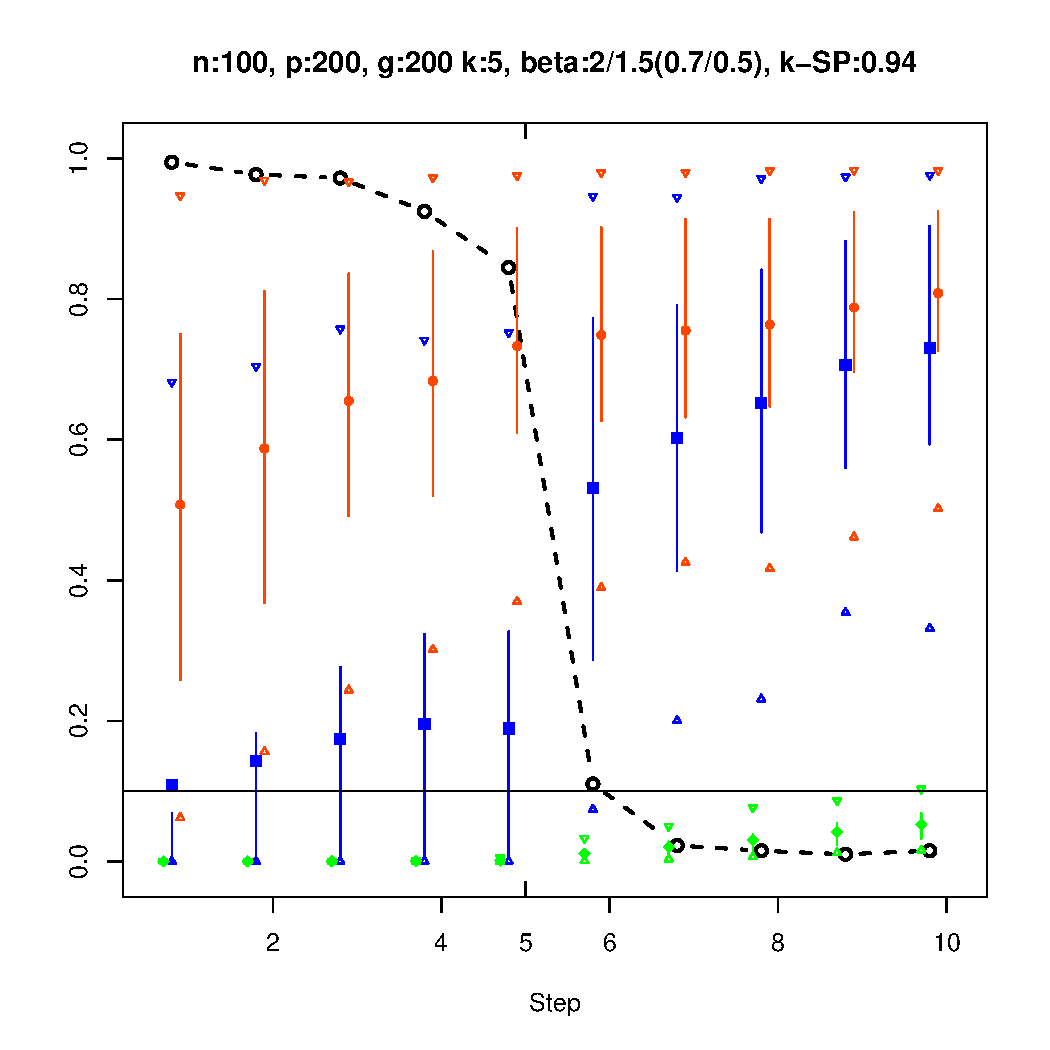
\includegraphics[width=0.5\textwidth]{../figs/gaussian_n100_p200_g200_k5_lower1pt5_upper2_corr0pt2_noisecorr0pt1.pdf}}
\hspace{-15pt}
\subfigure[Gaussian with groups]{
\label{fig:gaussgroups}
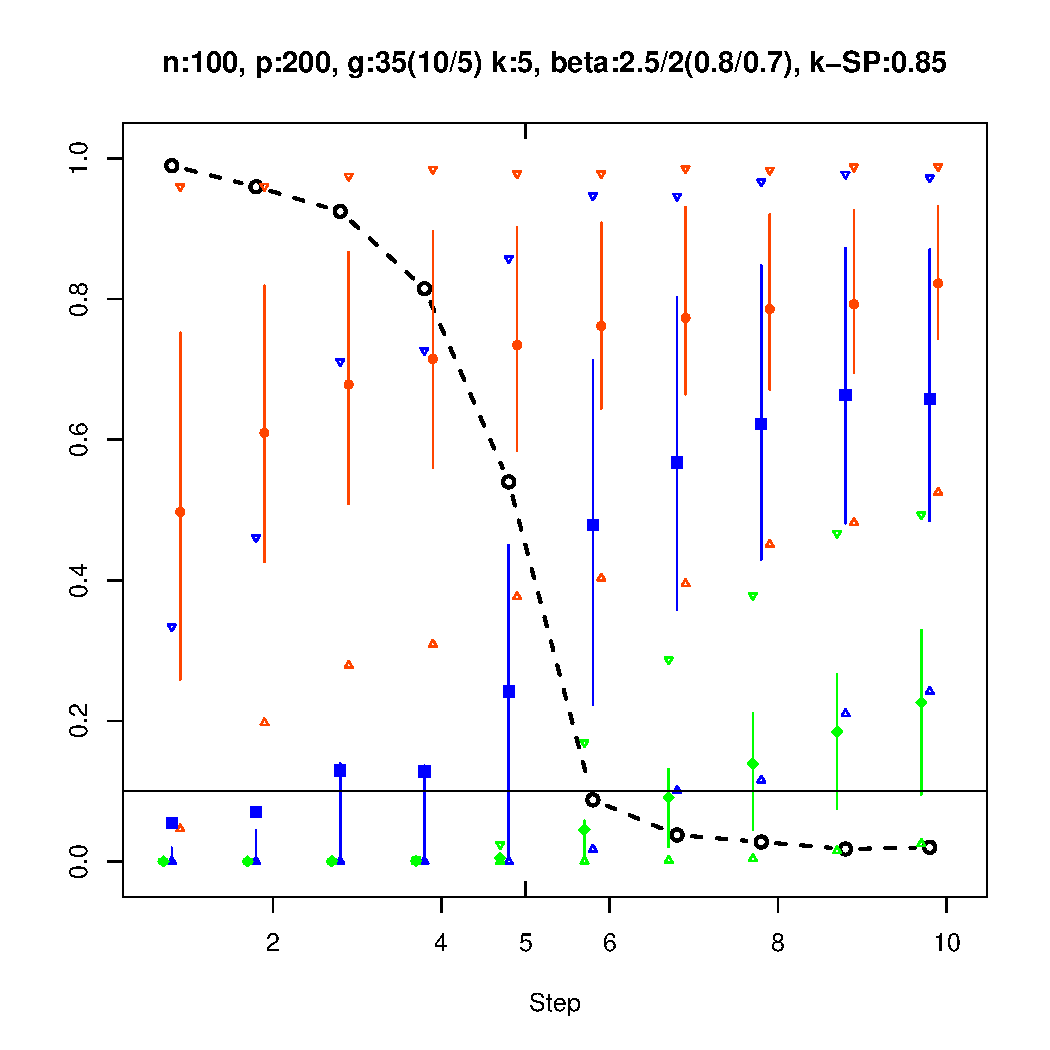
\includegraphics[width=0.5\textwidth]{../figs/gaussian_n100_p200_g35_k5_lower2_upper2pt5.pdf}}
\caption{\small \it The left panel shows results for Gaussian design
matrices with equicorrelation $\rho=0.2$ and equicorrelated noise with
correlation 0.1. The right panel shows results for an independent
Gaussian design with groups of sizes 5 and 10.}
\end{center}
\end{figure}


\input{../small_sim_selection.tex}

\input{../small_sim_estimation.tex}

\begin{figure}[h]
\begin{center}
\subfigure[Real data categorical design]{
\label{fig:hivnrti}
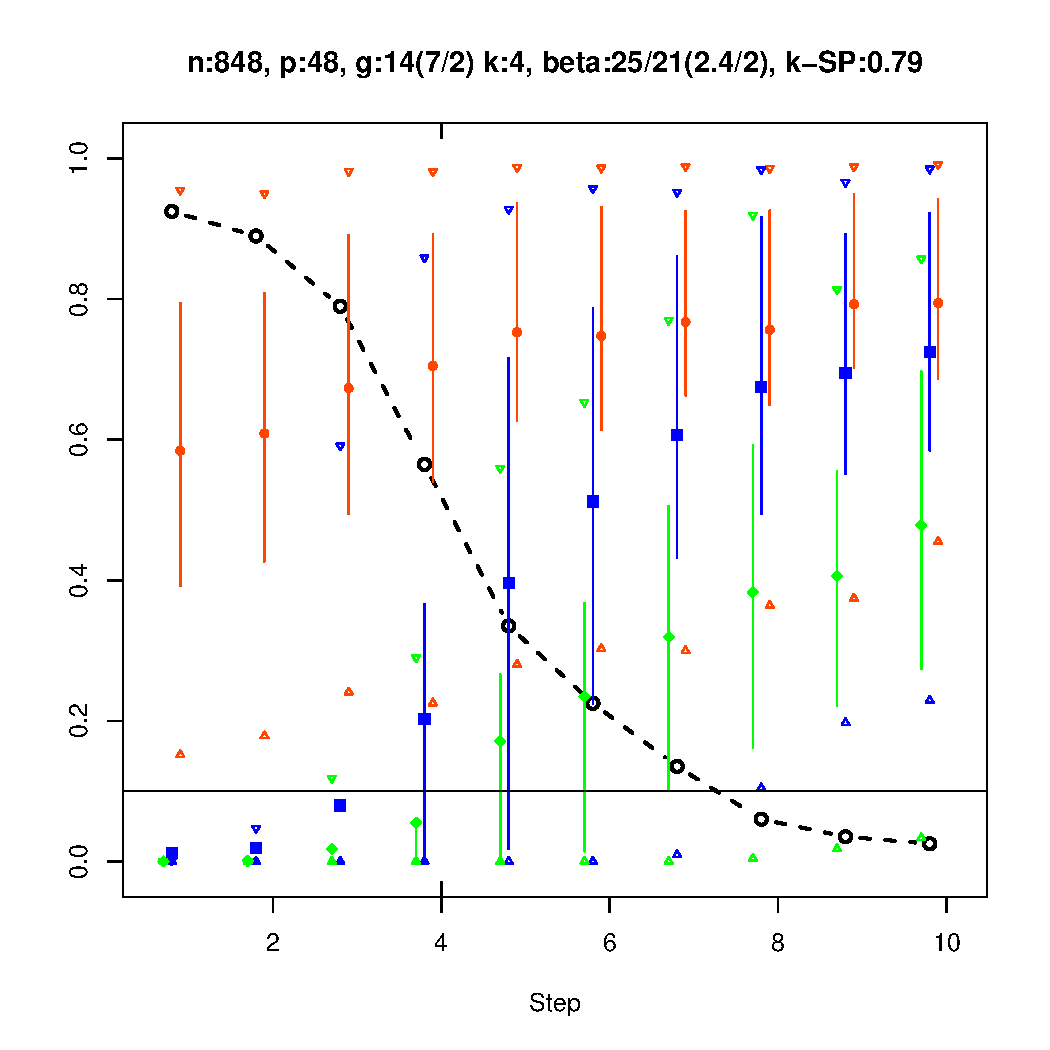
\includegraphics[width=0.5\textwidth]{../figs/HIV_NRTI_n848_p48_g14_k4_lower21_upper25.pdf}}
\hspace{-15pt}
\subfigure[Simulated categorical design]{
\label{fig:gausscat}
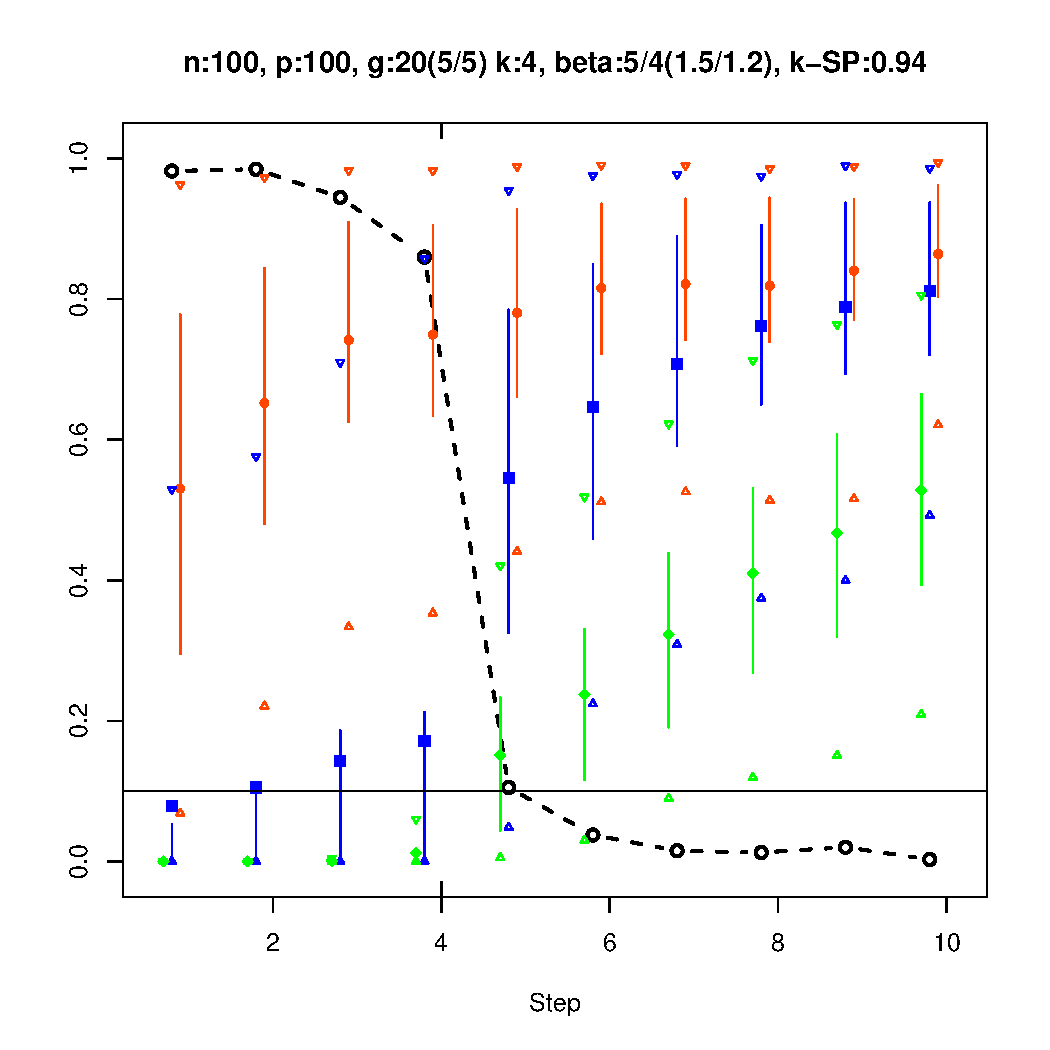
\includegraphics[width=0.5\textwidth]{../figs/categorical_n100_p100_g20_k4_lower4_upper5.pdf}}
\caption{\small \it The left panel shows results for a categorical design
taken from a real data set.
The right panel shows results for categorical matrices with all categories having 5 levels.}
\end{center}
\end{figure}

\input{../large_sim_selection.tex}




\section{Applications}
\label{sec:applications}
We now turn to applying forward stepwise and examining the behavior of
our test statistic in several unique settings, including a real data
example.


\subsection{Glinternet for hierarchical interactions}
\label{sec:glint}
In regression settings with many variables, considering models with pairwise interactions can drastically increase model complexity. \cite{glint} propose a method called \textsc{glinternet} to reduce the statistical complexity of this problem. The method imposes a strong hierarchical constraint on interactions (similar to that in \cite{bien:hierarchical}) where an interaction term can only be included if both its main effects are also included. They accomplish this by creating a design matrix with both main effects alone and also with groups including main effects with their first order interactions. Then they fit a group lasso model with the expanded design matrix. Because interaction terms only appear in groups along with their respective main effects, the hierarchy condition holds for the fitted model. We now consider a related procedure as an example problem, but first modify their method to simplify some parts. Let the expanded design matrix be given by
\begin{equation}
\label{eq:glintmat}
\tilde X = \begin{pmatrix} X_1 & \cdots & X_G & X_{1:2} & \cdots & X_{1:G} & X_{2:3} & \cdots & X_{(G-1):G}  \end{pmatrix}
\end{equation}
where $X_{g:h}$ is the submatrix including $X_g$, $X_h$, and all
$p_gp_h$  column multiples between columns in group $g$ and columns
in group $h$. For example, if
\[
X_g = \begin{pmatrix} X_{g1} & X_{g2} \end{pmatrix}, \quad
X_h = \begin{pmatrix} X_{h1} & X_{h2} \end{pmatrix}
\]
are two groups each containing two columns, then
\[
X_{g:h} = \begin{pmatrix} X_g & X_h & X_{g1} * X_{h1} & X_{g1} * X_{h2} & X_{g1} * X_{h1} & X_{g2} * X_{h2} \end{pmatrix}
\]
where * denotes the pointwise product (Hadamard product) of vectors
(the $i$th entry of $X_{g1} * X_{h1}$ is the $i$th entry of $X_{g1}$ times
the $i$th entry of $X_{h1}$). Note that this expanded matrix has
$\tilde G = G + \binom{G}{2} = O(G^2)$ groups. We refer to the first
$G$ of these as main effects or main effect groups, and the remaining
as interaction groups. Finally, instead of fitting a
model by group lasso, we use forward stepwise on the expanded design
matrix. The overlapping groups still guarantee that our fitted model
satisfies the strong hierarchy condition. 

%However, we must first modify our implementation of forward stepwise to prevent the possibility of including main effect groups after the main effects are already included in the model as part of an interaction group. To do this we compute the residual using the whole model in each step, rather than by subtracting the effect of the current group being included. For a set of group indices $A \subseteq \{ 1, \ldots G \}$ we write $X_A$ for the submatrix of the design matrix containing all the groups in $A$.
% \begin{algorithm}
% \DontPrintSemicolon
% \caption{\small \it Modification to compute residual from full model}
% \BlankLine
% \CommentSty{\# Everything the same as before, additionally:}\;
% %  $P_A \gets I - X_AX_A^\dagger$\;
% %  $r_s \gets P_A r_{s-1}$\;
% \If{$g^*$ is an interaction group}{
%   $g_1, g_2 \gets$ main effects groups of $g^*$\;
%   A^c \gets A^c \slash \{ g_1, g_2 \}\;
% }%\;
% %$r_s \gets y - \text{lsfit}(X_A, y)$\;
% \BlankLine
% \label{algo:fs:full}
% \end{algorithm}
% \begin{algorithm}
% \DontPrintSemicolon
% \KwData{An $n$ vector $y$ and $n \times p$ matrix $X$ of $G$ groups of variables}
% \KwResult{Active set $A$ of variable groups included in the model}
% \SetKwFunction{lsfitResidual}{lsfitResidual}
% \caption{\small \it Forward stepwise for glinternet}
% \BlankLine
% Compute design matrix~(\ref{eq:glintmat}) and expanded grouping $\tilde G$\;
% $A \gets \emptyset$\;
% $A^c \gets \{ 1, \ldots, G \}$\;
% $r_0 \gets y$\;
% \For{$s \gets 1$ \KwTo $steps$}{
%   $g^* \gets \argmax_{g \in A^c} \{ \norm{X_g^T r_{s-1}}_2 / w_g \}$\;
%   $P \gets I - X_{g^*}X_{g^*}^\dagger$\;
%   $A \gets A \cup \{ g^* \}$\;
%   $A^c \gets A^c \backslash \{ g^* \}$\;
%   \For{$g \in A^c$}{
%     $X_g \gets P X_g$\;
%   }
%   $r_s \gets P r_{s-1}$\;
% }
% \KwRet{$A$}
% \label{algo:fsgl}
% \end{algorithm}

To demonstrate this method by simulation, we constructed signals which have
the first $k/3$ main effects nonzero but with no interactions, and the
remaining $2k/3$ nonzero main effects are matched to each other to form
interactions.
This way each nonzero main effect with any nonzero interactions has
exactly one nonzero interaction. Furthermore, each nonzero interaction
coefficient has been inflated to be larger than the corresponding main
effect coefficients. This special case is favorable for our algorithm,
but our purpose here is merely to demonstrate the flexibility of the
hypothesis test and not to propose a general procedure for models with
interactions.

Results are shown in Figure~\ref{fig:glint}. The left
panel shows average power of forward stepwise. Power is calculated
using the group structure we impose, and not in terms of the original
main effects and interactions. However, the dotted line shows a more
forgiving definition of power where we are rewarded for discovering part
of a nonzero group, i.e. for discovering only one main effect from a
true interaction group. In the right panel we see that the global null
result still holds (red vertical lines), and that with a signal the
p-value is small until the signal has been recovered (blue). The
interaction power is the proportion of nonzero interaction groups
that were discovered and is labeled ``Int. Power.''

\begin{figure}
\begin{center}
\subfigure[Forward stepwise on glinternet]{
\label{fig:glint:fwd}
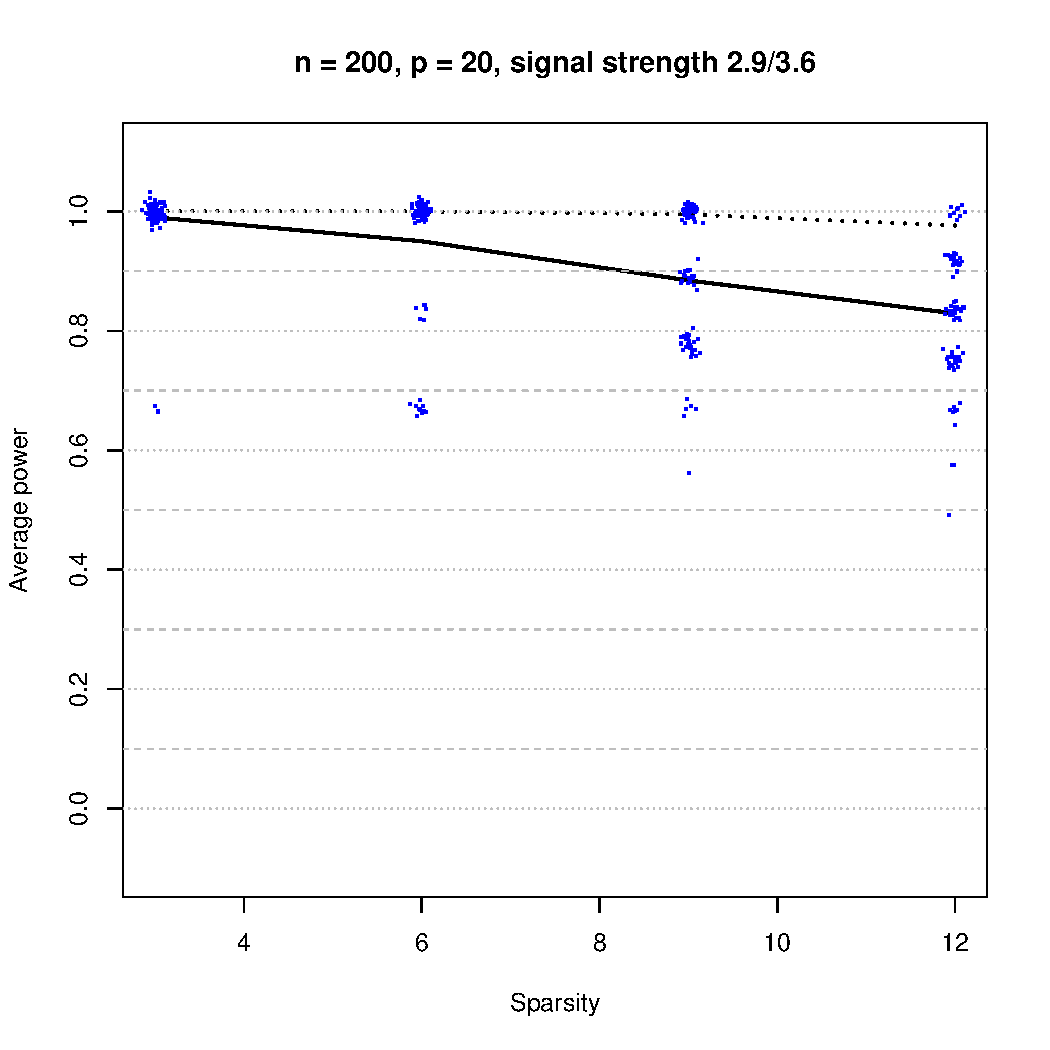
\includegraphics[width=0.5\textwidth]{../figs/fwdstep/gauss_glint_p20_n200_lower2p9_upper3p6.pdf}}
\hspace{-15pt}
\subfigure[P-value with glinternet]{
\label{fig:glint:pval}
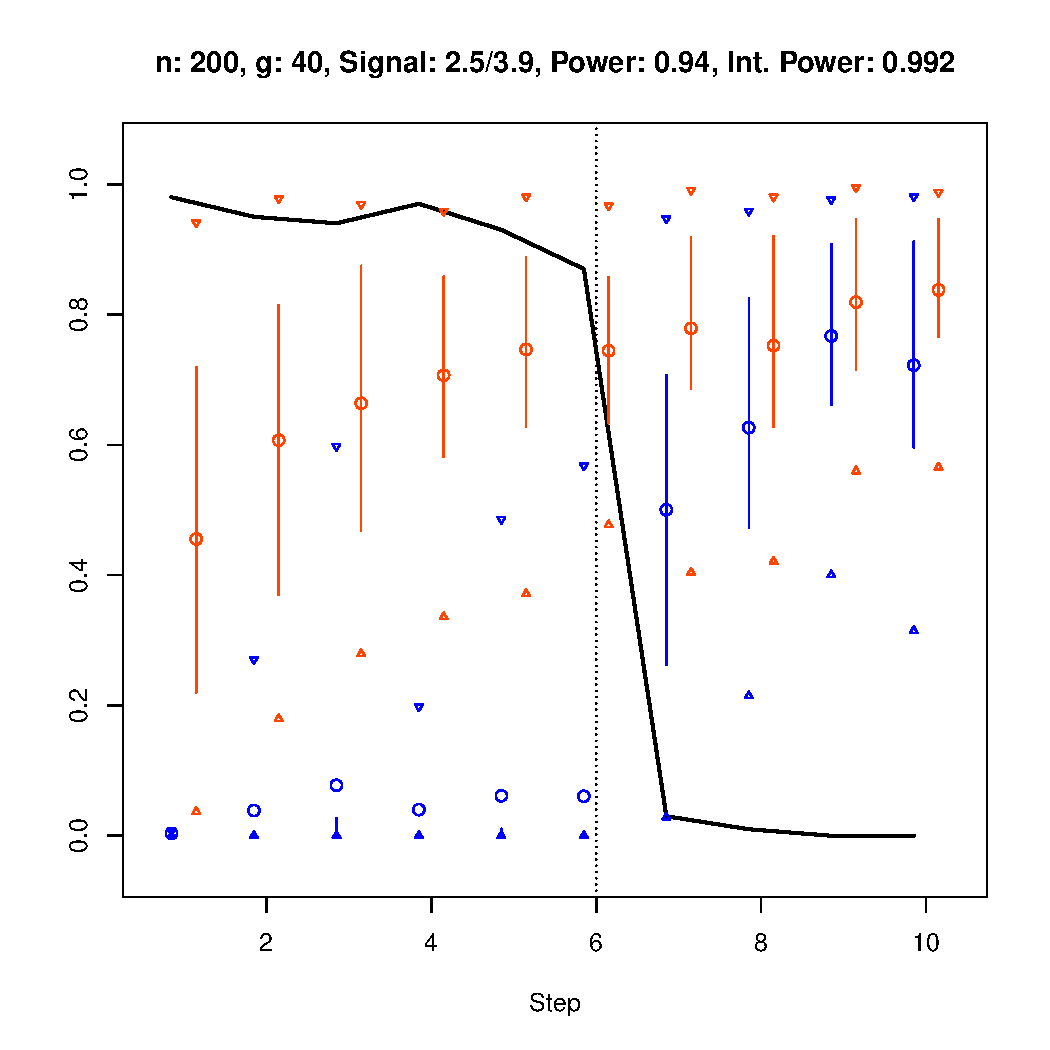
\includegraphics[width=0.5\textwidth]{../figs/gaussian_size1_n200_p40_g40_k6_lower2p5_upper3p9_glint.pdf}}
\caption{\small \it The left panel shows the power of forward stepwise
for various sparsity levels. The right panel shows our p-value marginally
over each step, with red indicating the global null case and blue
indicating a signal with $k=6$ nonzero groups.}
\label{fig:glint}
\end{center}
\end{figure}


\subsection{Generalized additive model selection}
\todo Finish code \\
\todo Write section \\

\subsection{Real data example}
\label{sec:hiv}
\todo Sanity check my analysis \\
\todo For rare mutations try binary wildtype/non-wt? \\
\todo Finish writing section \\

\cite{HIV} use genomic information to predict efficacy of antiretroviral
drugs in treating HIV. Quantitative measurements of drug
response/resistance were regressed on categorical covariates encoded
the presence and type of certain genetic mutations. We attempt a similar
analysis using forward stepwise, and report our P-value at each step.
Categorical covariates are encoded as groups of binary variables using
the full encoding, and weights are set to the square-root of the
number of levels for that covariate. We perform forward stepwise once
for each drug response, restricting to the subset of the data with
no missing values and requiring all categorical variables to have 2 or
greater observations in each level. 

\begin{figure}
\begin{center}
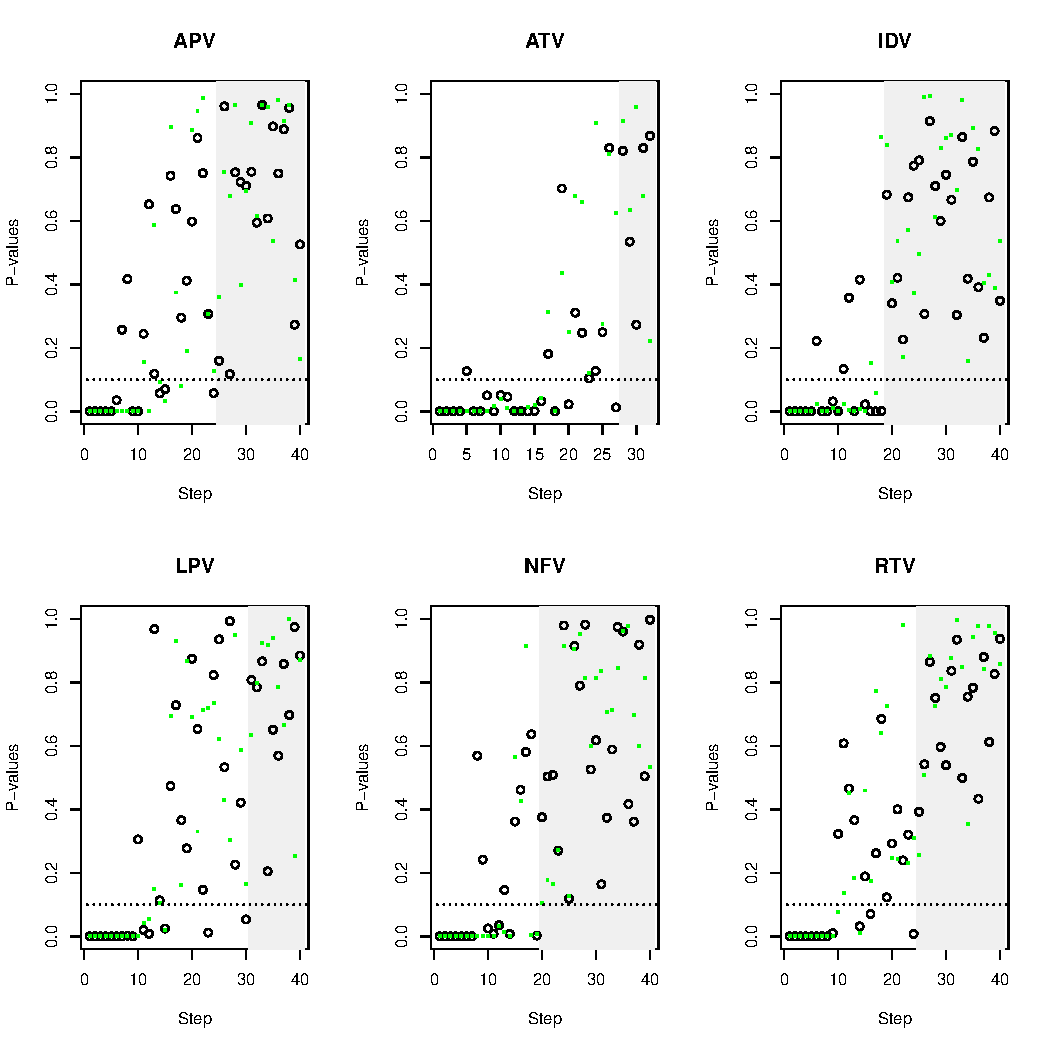
\includegraphics[width=0.9\textwidth]{../figs/HIV_PI.pdf}
\caption{\small \it Results from PI dataset}
\label{fig:HIVPI}
\end{center}
\end{figure}

\begin{figure}
\begin{center}
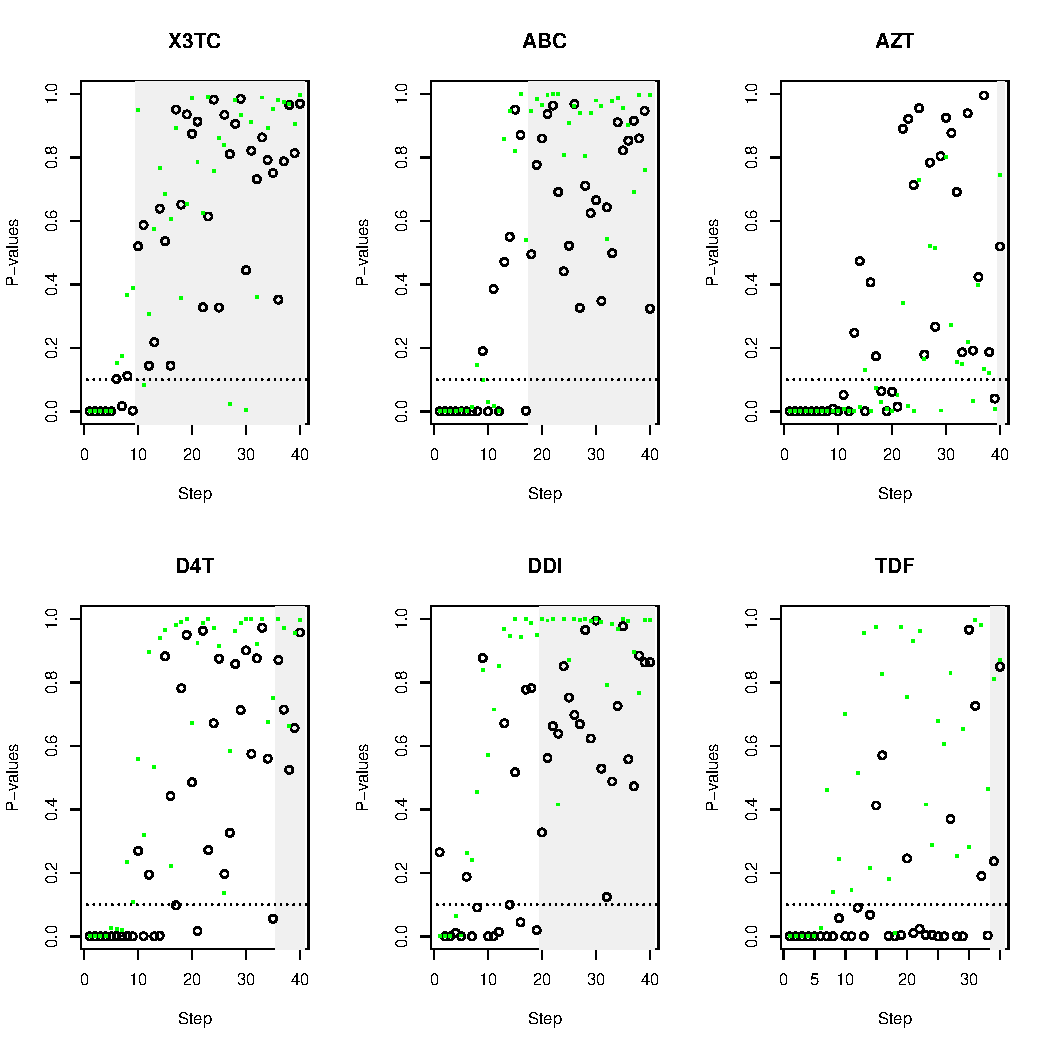
\includegraphics[width=0.9\textwidth]{../figs/HIV_NRTI.pdf}
\caption{\small \it Results from NRTI dataset}
\label{fig:HIVNRTI}
\end{center}
\end{figure}

Results from two data sets are displayed in Figure~\ref{fig:HIVPI} and
Figure~\ref{fig:HIVNRTI}. The PI data contains protease inhibitor
resistance mutations, and the NRTI data contains nucleoside RT inhibitor
resistance mutations.
Each panel shows results for a different drug,
with p-values plotted by step in forward stepwise. The solid black point
is the last p-value to fall under the 0.1 threshold and points after it
are colored red. If the \textit{last} stopping rule were used then the
p-values for including variables are the black points, and the resulting
models are shown in Tables 4 and 5. (\todo Fix this ref after re-running)

%\begin{figure}
%\begin{center}
% latex table generated in R 3.0.2 by xtable 1.7-1 package
% Wed May 14 17:30:50 2014
\begin{table}[ht]
\centering
\begin{tabular}{rllll}
  \hline
 & Drug & n & G & Selected variables \\ 
  \hline
1 & APV & 768 & 82 & P90 P46 P54 P84 P88 P32 P50 P76 P33 P10 P15 P82 P93 P24 P47 P64 P58 P11 P43 P35 P77 P63 P13 P48 \\ 
  2 & ATV & 329 & 71 & P90 P54 P84 P50 P30 P32 P24 P76 P62 P46 P35 P88 P82 P73 P58 P43 P77 P48 P64 P36 P13 P14 P74 P71 P11 P57 P20 \\ 
  3 & IDV & 827 & 82 & P90 P46 P54 P84 P82 P62 P88 P73 P35 P50 P71 P24 P76 P32 P48 P10 P20 P63 \\ 
  4 & LPV & 517 & 76 & P90 P54 P46 P84 P36 P82 P76 P47 P50 P10 P73 P33 P53 P24 P48 P62 P93 P11 P71 P60 P14 P19 P20 P41 P70 P13 P16 P37 P88 P30 \\ 
  5 & NFV & 844 & 82 & P90 P46 P30 P54 P84 P36 P88 P73 P24 P82 P50 P71 P10 P74 P77 P35 P63 P20 P48 \\ 
  6 & RTV & 795 & 82 & P90 P54 P46 P84 P82 P36 P24 P50 P32 P73 P13 P15 P88 P30 P35 P33 P93 P71 P10 P58 P53 P63 P48 P20 \\ 
  7 & SQV & 826 & 82 & P90 P84 P54 P30 P48 P36 P24 P53 P88 P73 P15 P82 P10 P71 P76 P58 P93 P74 P50 P63 P62 P20 P14 P41 P46 P32 P57 P70 P67 P43 P13 P16 \\ 
   \hline
\end{tabular}
\caption{Variables chosen using \textit{last} stopping rule in forward stepwise} 
\end{table}


%\label{tab:HIVPI}
%\end{center}
%\end{figure}

%\begin{figure}
%\begin{center}
% latex table generated in R 3.0.2 by xtable 1.7-1 package
% Mon May  5 22:18:44 2014
\begin{table}[ht]
\centering
\begin{tabular}{rllll}
  \hline
Drug & n & G & $\hat k$ & Selected variables \\ 
  \hline
X3TC & 633 & 176 & 9 & P184 P41 P65 P67 P151 P210 P181 P83 P215 \\ 
ABC & 628 & 176 & 17 & P184 P41 P151 P67 P210 P65 P74 P83 P218 P215 P115 P69
\ldots  \\% P60 P43 P202 P200 P219 \\ 
AZT & 630 & 176 & 39 & P41 P67 P184 P151 P210 P70 P74 P215 P181 P77
P103 P69 \ldots \\ % P203 P218 P135 P100 P196 P35 P43 P219 P208 P98 P118 P221 P83 P169 P142 P178 P227 P162 P60 P65 P121 P21 P111 P44 P68 P108 P94 \\ 
D4T & 630 & 176 & 35 &P41 P151 P67 P210 P184 P69 P65 P218 P215 P118 P75 P83
\ldots \\ % P219 P181 P214 P77 P203 P20 P122 P40 P44 P70 P103 P221 P90 P119 P116 P74 P6 P177 P35 P100 P200 P94 P85 \\ 
DDI & 632 & 176 & 19 & P184 P151 P41 P74 P65 P67 P210 P218 P83 P75 P69
P118
\ldots \\ % P214 P215 P179 P106 P123 P70 P219 \\ 
TDF & 353 & 153 & 33 &P41 P184 P70 P210 P65 P74 P181 P62 P215 P68 P67 P98
\ldots \\ %P35 P151 P196 P202 P75 P118 P135 P218 P203 P122 P6 P115 P69 P103 P60 P121 P21 P77 P39 P142 P100 \\ 
   \hline
\end{tabular}
\caption{Variables chosen using \textit{last} stopping rule in forward
  stepwise on HIVdb NRTI dataset} 
\label{tab:hivNRTI}
\end{table}


%\label{tab:HIVNRTI}
%\end{center}
%\end{figure}

\section{Discussion}
\label{sec:discuss}

\todo Brief summary \\
\todo After finising everything else, move some points of discussion
here \\
\todo Mention ongoing work, like tracking all the constraints to
get an exact p-value at every step. \\

\newpage

\bibliographystyle{ims}
%\bibliographystyle{acmtrans-ims}
\bibliography{paper}

\newpage

\appendix
\section{Derivation of closed forms of statistic}
\label{app:closedform}

\todo Clean this section \\
\todo Make $M=\lambda_2$ a special case corollary \\

For the sake of completeness this appendix provides full derivations
of closed forms for the quantities required to compute our
statistic. We require two facts from \cite{tests:adaptive}

A point $\eta \in \K$ maximizes $f_\eta$ over a convex
set $\K$ if and only if the following conditions hold: 
\begin{equation}
\label{eq:maxcond}
\grad f_{|T_{\eta}\K} = 0, \quad
\tf^{\eta}_{\eta} \geq \V^+_{\eta}, \quad
\tf^{\eta}_{\eta} \leq \V^-_{\eta}, \quad \text{and} \quad
\V^0_{\eta} \leq 0.
\end{equation}
The same equivalence holds true even when $\K$ is only locally
convex. 

Write $M^{\pm}_{\eta, h}$ and $M^0_{\eta, h}$ as the corresponding suprema and infima over the restricted parameter set $S_h$. Note that the characterization of the global maximizer (Lemma 1, general paper) implies $M^0_{\eta, h} \leq 0$ and $M^+_{\eta, h} \leq M^-_{\eta, h}$ for all $h \neq g$. This will be used below to eliminate some degenerate cases of the optimization sub-problem on each $S_h$.

Now fix $h$, let $P_g = X_gX_g^T$ and define
\begin{align*}
a_h &= w_h^{-1} X_h^T (I-P_g) y \\
b_h &= w_g w_h^{-1} X_h^T P_g y / \norm{X_g^T y} \\
c_h &= a_h^T b_h / (\norm{a_h} \norm{b_h}) \\
K_h   &= \{ x : \norm{x} = 1, b_h^Tx > w \}
\end{align*}
Note that $K_h = \emptyset$ if and only if $\norm{b_h} < w$. We consider two cases. First, suppose $\norm{b_h} > w$. In this case we must rule out one sub-case, when $a_h$ is not in the polar cone of $K_h$. If this occurs, then on at least one side of the boundary of $K_h$ we have $a_h^Tx > 0$ there, so that the infimum inside $K$ is $-\infty$ but the supremum outside $K$ is $+\infty$. This violates the characterization of the global maximizer of the original process as described above, so this case cannot occur.

Now, if $a_h$ is in the polar cone of $K_h$ (and ruling out the probability zero case where $a_h^Tx = 0$ on the boundary of $K_h$), then the numerator $a_h^Tx < 0$ on $K_h$ so there is a finite positive infimum in the interior $K_h$. Similarly there is a finite positive supremum on the interior of $K_h^c$ (the numerator is negative near the boundary of $K_h$ by continuity).

To attain the infimum on $K_h$ requires making $x$ close to $b_h$ and simultaneously making the numerator closer to zero, so $x$ should be on the side of $b_h$ that is closer to $a_h$. To attain the supremum on $K_h^c$ requires making $x$ simultaneously close to $a_h$ (so that $a_h^Tx > 0$) and $b_h$ (to make the denominator small). In summary, both the infimum and supremum are attained with $x$ between $a_h$ and $b_h$, when the angle $\theta$ between $a_h$ and $b_h$ is larger than both the angle $\psi$ between $a_h$ and $x$ and the angle $\phi$ between $x$ and $b_h$. This allows the simplification $\phi = \theta - \psi$. This is easier to verify for the case when $\norm{b_h} < w$.

We have verified that solving both cases requires finding the maxima of the trigonometric form $\norm{a_h} \cos (\psi) / (w - \norm{b_h} \cos(\theta - \psi))$ of the linear fraction on the interiors of $K_h$ (if it is nonempty) and $K_h^c$. The derivative is proportional to
\[
\frac{\norm{b_h} \sin(\theta) - w \sin(\psi)}{w - \norm{b_h} \cos(\theta - \psi)}
\]
Since we have ruled out the boundary of $K_h$, we can ignore the denominator and focus on critical points corresponding to the angles $\psi^{\pm}$ (symmetric about $\pi/2$) where $\sin(\psi^{\pm}) = (\norm{b_h} / w) \sin (\theta)$. That is,
\[
\psi^{\pm} \in \arcsin \frac{\norm{b_h}}{w} \sqrt{1-c_h^2}
\]
Note that these critical points only exist if $\sin(\theta) < w/\norm{b_h}$, and since we have argued that the infimum and supremum are attained it follows that this condition is met in our case. Let $\psi^+$ denote the smaller of the two angles. If $K_h$ is nonempty, then $\psi^-$ gives the infimum in $K_h$ and $\psi^+$ the supremum on $K_h^c$. This is necessary since if $x$ is in $K_h$ then its angle from $a_h$ is larger than $\pi/2$ because $a_h$ is in the polar cone of $K_h$. If $K_h$ is empty, then the supremum is still attained at $\psi^+$ since the numerator is negative at $\psi^- > \pi/2$ and the denominator is always positive.

Finally we calculate the values of the linear fraction at $\psi^{\pm}$. Let us first record some facts:
\begin{align*}
0 < \psi^+ < \pi/2, \quad \psi^- = \pi - \psi^+ \\
\cos(\theta) = c_h, \quad \sin(\theta) = \sqrt{1-c_h^2} \\
\sin(\psi^+) = \sin(\psi^-) = \frac{\norm{b_h}}{w} \sin(\theta) \\
\cos(\psi^+) = -\cos(\psi^-) = \sqrt{1 - (\norm{b_h}/w)^2(1-c_h^2)}
\end{align*}
Using the angle difference formula,
\begin{align*}
\cos(\theta - \psi^+) & = \frac{\norm{b_h}}{w} (1-c_h^2) +  c_h \cos(\psi^+) \\
& = \frac{\norm{b_h}}{w} (1-c_h^2) +  c_h \cos(\psi^+)
\end{align*}
Hence
\begin{align*}
M^+_{\eta, h} & = \frac{ \norm{a_h} c_h }{ w - (\norm{b_h}^2/w) (1-c_h^2) - \norm{b_h} c_h \cos(\psi^+) } \\
% & = 
% & = \frac{ w \norm{a} a_h^Tb_h / \norm{b_h} }{ w^2 - \norm{a}\norm{b}^2 + (a^Tb)/\norm{a} - a^Tb \cos \psi^+ }
\end{align*}
And $M^-_{\eta, h}$ is $\infty$ when $\norm{b_h} < w$ and otherwise given by
\begin{align*}
M^+_{\eta, h} & = \frac{ \norm{a_h} c_h }{ w - (\norm{b_h}^2/w) (1-c_h^2) + \norm{b_h} c_h \cos(\psi^+) } \\
\end{align*}

I haven't been able to algebraically simplify these yet to a form that allows my $\lambda_2$ proof below to go through. The version below just assumes $\norm{b_h} < w = 1$.

\hrule
\hrule
We can rewrite this by rationalizing the denominator:
\[
M =
\frac
{ a_h^T b_h +  \sqrt{ a_h^T a_h (1-b_h^Tb_h) + (a_h^T b_h)^2 }  }
{ 1-b_h^Tb_h }
\]
Leaving $M$ in this form we now consider $\lambda_2$. The KKT conditions for the group lasso problem give (directly from Yuan and Lin)
\begin{align*}
\norm{ X_g^T(y - X \beta) } & \leq \lambda w_g \quad \forall \beta_g \neq 0 \\
\beta_g & = \left( 1 - \frac{ \lambda w_g }{ \norm{S_g} } \right)_+ S_g
\end{align*}
where $S_g = X_g^T(y - X \beta_{-g})$. These expressions simplify for $\lambda_2 \leq \lambda < \lambda_1$. Letting $g$ be the index of the first group to enter we now have $S_g = X_g^Ty$ 
\begin{align*}
\beta_g & = \left( 1 - \frac{ \lambda w_g }{ \norm{X_g^Ty} } \right) X_g^Ty \\
\lambda w_h & \geq \norm{ X_h^Ty - X_h^T P_g y (1-\lambda w_g / \norm{X_g^Ty})  } \quad \forall h \neq g
\end{align*}
Now let $\lambda = \lambda_2$, so the inequality above is strict for all other groups and equality is attained for the second group to enter. Hence $\lambda_2$ satisfies
\begin{align*}
\lambda_2 & = \max_{h \neq g} 
\norm{ X_h^T(I - P_g) y - \lambda_2 ( w_g X_h^T P_g y / \norm{X_g^Ty} )  } / w_h\\
& = \max_{h \neq g} \norm{ a_h - \lambda_2 b_h } 
\end{align*}

Write $\lambda_{2,h}$ as the positive root of the quadratic equation obtained by squaring the norm, so $\lambda_{2,h}^2 = \norm{ a_h - \lambda_2 b_h }^2$. Then $\lambda_2 = \max_{h \neq g} \lambda_{2,h}$. Solving this (note that $b_h^Tb_h < 1$), we find
\[
\lambda_{2,h} = \frac
{ a_h^T b_h +  \sqrt{ a_h^T a_h (1-b_h^Tb_h) + (a_h^T b_h)^2 }  }
{ 1-b_h^Tb_h }
\]
Hence when $h$ is the index of the second group to enter, we have $\lambda_2 = \lambda_{2,h} = M$.

\end{document}

